%!TEX root = ../main.tex

El curso de Introducción al Análisis Real es uno de los más pesados en la carrera de matemáticas y los estudiantes carecen casi que de toda ayuda (no hay monitorias y los espacios en clase a veces son insuficientes), por estos motivos decidimos hacer este solucionario de las notas de Introducción al Análisis Real de los profesores Leonardo Rendón y Serafín Bautista, esto más que un solucionario es una guía de lectura de las notas, aquí encontrarás muchos de los conceptos o ideas del curso desde un punto de vista más de estudiante que ha sufrido esa materia y que sabe lo compleja que puede llegar a ser.\\

Esperamos que las soluciones de los ejercicios que aportamos acá sirvan de guía para entender los conceptos y mecanismos que se deben usar para atacar este tipo de problemas.\\

Muchos éxitos - mmanosalva y eochoaq

\section{Algunos ejercicios al lector: }

\begin{itemize}[leftmargin=*]
    \item  Probar que $(\mathbb{R}^n,d_1)$ y $(\mathbb{R}^n,d_{\infty})$ son espacios métricos.\\

    \begin{proof}
        $\bullet$ Sean $p,q \in \mathbb{R}^n$, tenemos que:

        $$d_1(p,q)=\sum_{k=1}^n|p_k-q_k|$$

        Luego como $|p_k-q_k|\geq 0 $, $d_1(p,q)\geq 0$ (estamos sumando valores positivos). Ahora si $d_1(p,q)=0$, como $|p_k-q_k|\geq 0$ entonces $|p_k-q_k|=0$ para todo $k$, luego $p_k=q_k$ para todo $k$, es decir $p=q$, además note que 

        $$d_1(p,q)=\sum_{k=1}^n|q_k-p_k|=d_1(q,p)$$

        Esto ya que $|p_k-q_k|=|q_k-p_k|$, Ahora veamos la desigualdad triangular.

            \begin{align*}
                d_1(p,q)&=\sum_{k=1}^n|p_k-q_k|\\
                &=\sum_{k=1}^n|p_k-q_k+r_k-r_k|\\
                &\leq \sum_{k=1}^n|p_k-r_k|+\sum_{k=1}^n|r_k-q_k|=d_1(p,r)+d_1(r,q)
            \end{align*}
            
            $\bullet$ Nuevamente tomamos $p,q \in \mathbb{R}^n$, tenemos que:

        $$d_{\infty}(p,q)=\max_{1\leq k\leq n}|p_k-q_k|$$

        como $|p_k-q_k|\geq 0$ pues es claro que el máximo será mayor igual que 0 y por tanto $d_{\infty}(p,q)\geq 0$. Como $|p_k-q_k|=|q_k-p_k|$:

         $$d_{\infty}(p,q)=\max_{1\leq k\leq n}|q_k-p_k|=d_{\infty}(q,p)$$

         Ahora si $max_{1\leq k \leq n} |q_k-p_k|=0$, $|p_k-q_k|=0$ para todo $k$ (si el máximo el 0 los demás también por definición de máximo) y como $|p_k-q_k|=0$ para todo $k$, pues $p_k=q_k$ para todo k, es decir $p=q$. Veamos la desigualdad triangular.

            \begin{align*}
                d_{\infty}(p,q)&=\max_{1\leq k\leq n}|p_k-q_k|\\
                &=\max_{1\leq k\leq n}|p_k-q_k+r_k-r_k|\\
                &\leq \max_{1\leq k\leq n}|p_k-r_k|+\max_{1\leq k\leq n}|r_k-q_k|\\
                &\leq d_{\infty}(p,r)+d_{\infty}(r,q)
            \end{align*}
        
    \end{proof}

 

    \item Sea $X$ un conjunto no vacío y $f: X \rightarrow \mathbb{R}$. Diremos que $f$ es una función acotada si existe $k>0$ tal que para todo $x \in X$ se tiene $|f(x)| \leq k$. Consideremos el conjunto $B(X)=\{f: X \rightarrow \mathbb{R}: f$ es acotada $\}$. Definamos:

        $$
        \begin{aligned}
        d: B(X) \times B(X) & \rightarrow \mathbb{R} \\
        (f, g) & \mapsto d(f, g)
        \end{aligned}
        $$

        donde $d(f, g)=\sup \{|f(x)-g(x)|: x \in X\}=\sup _{x \in X}|f(x)-g(x)|$. Entonces $(B(X), d)$ es un espacio métrico.\\

        \begin{proof}
            Es inmediato que $d(f,g)\geq 0$ por definición de supremo y porque $|f(x)-g(x)|\geq 0$. Como $|f(x)-g(x)|=|g(x)-f(x)|$, entonces también se tiene que $d(f,g)=d(g,f)$.

            Tenemos que $|f(x)-g(x)|\geq 0$, luego por definición de supremo si $\sup_{x \in X}|f(x)-g(x)|=0$, entonces $|f(x)-g(x)|=0$ para todo $x\in X$, así $f=g$, o sea si $d(f,g)=0$, entonces $f=g$. Veamos ahora la desigualdad triangular :
            \begin{align*}
                d(f,g)&=\sup_{x\in X}|f(x)-g(x)|\\
                &=\sup_{x\in X}|f(x)-g(x)+h(x)-h(x)|\\
                &\leq \sup_{x\in X}|f(x)-h(x)|+|h(x)-g(x)|\\
                &=\sup_{x\in X}|f(x)-h(x)|+\sup_{x\in X}|h(x)-g(x)|\\
                &=d(f,h)+d(h,g)
            \end{align*}

            Esto ya que $\sup (A+B)=\sup(A)+\sup (B)$\\
            
        \end{proof}

        \item  Dado $(E, d)$ un espacio métrico, toda bola abierta es un conjunto abierto. En efecto, dados $B_E(p, r)$ (con $r>0$ y $\left.p \in E\right)$ y $q \in B_E(p, r)$, tomamos $r^{\prime}=r-d(p, q)$ de donde se tiene que $B_E\left(q, r^{\prime}\right) \subset B_E(p, r)$ (verifique esta contenencia como ejercicio).\\
       
        \begin{proof}
            Sea $x \in B_E(q,r^{\prime})$, entonces:

            \begin{align*}
                d(p,x)&\leq d(p,q)+d(q,x)\\
                &\leq r-d(q,x)+d(q,x)\\
                &\leq r
            \end{align*}

         Luego el punto $x\in B_E(p,r)$ y se tiene la contenencia\\
        \end{proof} 

Note que la prueba no debe depender del dibujo, sin embargo hacer dibujos puede ser de ayuda para tener una idea de la demostración, como ocurrió en este caso

\begin{theorem}[Teorema 9]

Dado $(E,d)$ en espacio métrico, tenemos que:

\begin{itemize}
\item[1)]$E$ es cerrado

\item[2)] $\emptyset$ es cerrado

\item[3)] Unión finita de cerrados es cerrada.

\item[4)]Intersección arbitraria de cerrados es cerrada.

\end{itemize}
\end{theorem}
\vspace*{0.3cm}
\begin{proof}

\begin{itemize}
\item Note que $E^C=$ $\emptyset$ luego el complemento de $E$ es abierto. 

\item Por definición $E$ es abierto, luego $\emptyset$ es cerrado.

\item Consideremos $C_i$ una familia de cerrados, luego

$$\left(\bigcup_{i=1}^n C_i\right)^C=\bigcap_{i=1}^n C_i^C$$

Y como intersección finita de abiertos es abierto, entonces acabamos.

\item Nuevamente consideremos $C_i$ una familia de cerrados, entonces:

$$\left(\bigcap_{i \in I}C_i\right)^C=\bigcup_{i\in I}C_i^C$$

Y como unión arbitraria de abiertos es abierto, entonces acabamos.

\end{itemize}

\end{proof}



\end{itemize}

\begin{itemize}[leftmargin=*]
\item Sea $(E,d)$ un espacio métrico $\{p\}=\bigcap_{r>0} B[p, r]$\\

\begin{proof}
Suponga que $\{p\}\neq \bigcap_{r>0} B[p, r]$, luego existe $x\in \bigcap_{r>0} B[p, r]$ tal que $x\neq p$, entonces $x \in B[p,r]$ para todo $r>0$, pero $x\neq p$, por tanto $d(x,p)>0$, así existe $0<r<d(x,p)$ tal que $x\not \in B[p,r]$, contradicción.
 \end{proof}
\end{itemize}


\subsection{Quiz 4:}

\begin{itemize}[leftmargin=*]
\item  $\mathbb{Q}$ es abierto en $\left(\mathbb{R}, d_1\right)$.

\textbf{Falso: }Observamos que vía la definición de abierto $\mathbb{Q}$ no puede ser abierto ya que toda bola con centro en un racional va a tener irracionales dentro que no están en $\mathbb{Q}$ y por tanto la bola no está contenida en $\mathbb{Q}$, luego no es abierto.

De hecho es la forma de argumentar esto, vía la densidad de $\mathbb{Q}$ en $\mathbb{R}$ que ya conocemos de los cursos anteriores.

De manera más formal para todo $r>0$, $B(q,r)=(q-r,q+r) \not \subseteq \mathbb{Q}$, ya que $\mathbb{Q}$ es denso en $\mathbb{R}$.

Esto ocurre ya que estamos tomando bolas en $\mathbb{R}$. (Este argumento es para la métrica usual).

\item  $\mathbb{Q}$ es abierto en $\left(\mathbb{R}, d_d\right)$.\\

\begin{proof}
    Sea $q \in \mathbb{Q}$, consideremos $B(q,\frac{1}{2})$ entonces como estamos en la métrica discreta $B(q,\frac{1}{2})=\{x\in \mathbb{R}:d_d(q,x)<\frac{1}{2}\}=\{q\}$ por definición de la métrica y como podemos hacer esto para todo $q\in \mathbb{Q}$ y un conjunto es abierto si y solo si es unión de bolas abiertas, razonando inductivamente acabamos.
\end{proof}


\item $B\left(0, \frac{1}{2}\right)=B\left[0, \frac{1}{4}\right]$ en $\left(\mathbb{R}, d_d\right)$.\\

\textbf{Verdadero: }$B(0,\frac{1}{2})=\{x\in \mathbb{R} : d_d(0,x)<\frac{1}{2}\}=\{0\}=\{x \in \mathbb{R} : d_d(0,x)\leq \frac{1}{4}\}=B[0,\frac{1}{4}]$

\item $\mathbb{N}$ es cerrado en $\left(\mathbb{R}, d_1\right)$.\\

\begin{tikznt}
\centering
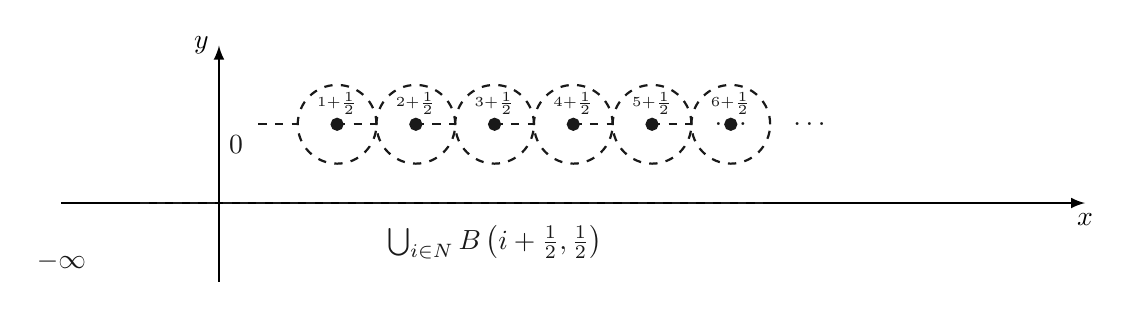
\begin{tikzpicture}
% Eje horizontal
\draw[-latex] (-2,0) -- (11,0) node[below]{$x$};

% Eje vertical
\draw[-latex] (0,-1) -- (0,2) node[left]{$y$};

% Intervalo (-\infty,0)
\node[black!90,below] at (-2,-0.5) {$-\infty$};
\node[black!90,above right] at (0,0.5) {$0$};

% Bolas alrededor de los números naturales
\foreach \x in {1,...,6}
{
\draw[thick,black!90,dashed] (\x+0.5,1) circle (0.5);
\filldraw[black!90] (\x+0.5,1) circle (2pt) node[font=\tiny, above] {\x$+\frac{1}{2}$};
}

% Unión de bolas
\draw[thick,black!90,dashed] (0.5,1) -- (1,1) (1.5,1) -- (2,1) (2.5,1) -- (3,1) (3.5,1) -- (4,1) (4.5,1) -- (5,1) (5.5,1) -- (6,1) (-1,0) -- (7,0);
\node[black!90] at (6.5,1) {$\ldots$};
\node[black!90] at (3.5,-0.5) {$\bigcup_{i\in\mathbb{N}} B\left(i+\frac{1}{2},\frac{1}{2}\right)$};
\node[black!90] at (7.5,1) {$\ldots$};

\end{tikzpicture}
\end{tikznt}

\begin{proof}
    Para ver que los naturales son cerrados con $d_1$, veamos que su complemento es abierto. Observe que:

    $$\displaystyle \mathbb{R}\setminus\mathbb{N}=(-\infty,0)\bigcup_{i \in \mathbb{N}}B\left(i+\frac{1}{2},\frac{1}{2}\right)$$

Note que esas bolas son abiertas y unión arbitraria de abiertos es abierto, efectivamente esas bolas cubren $\mathbb{R}\setminus \mathbb{N}$ entonces acabamos.
    
\end{proof}


\item Todo conjunto es abierto y cerrado en $\left(\mathbb{R}, d_d\right)$.\\

\begin{proof}
    Sea $X\subseteq R$ en $(R,d_d)$, $X$ es abierto ya que:

    $$X=\bigcup_{x \in X}B\left(x,\frac{1}{2}\right)$$

    Y $\mathbb{R}\setminus X$ también ya que:

     $$\mathbb{R}\setminus X=\bigcup_{j \in \mathbb{R}\setminus X}B\left(j,\frac{1}{2}\right)$$

     Luego $X$ es cerrado ya que su complemento es abierto, estos conjuntos los llamaremos \textbf{clopen} para simplificar en algunos casos.
\end{proof}

Note que podemos escoger cualquier $r\leq 1$ y la prueba se mantiene.

\item  El conjunto $\left[0, \frac{1}{4}\right)$ es cerrado en $\left(\left[0, \frac{1}{2}\right),\left.d_1\right|_{\left[0, \frac{1}{2}\right) \times\left(0, \frac{1}{2}\right)}\right)$\\

\textbf{Falso: }Queremos ver que $[0,\frac{1}{4})^C=[\frac{1}{4},\frac{1}{2})$ no es abierto, note que $B(\frac{1}{4},r)=(\frac{1}{4}-r,\frac{1}{4}+r)$ para todo $r>0$ no está contenida en $[\frac{1}{4},\frac{1}{2})$, entonces $[0,\frac{1}{4})$ no es cerrado en $([0,\frac{1}{2}),d|_{[0,\frac{1}{2})\text{x}[0,\frac{1}{2})})$ 

\item  Sean $(E, d)$ un espacio métrico, $A \subset E_1 \subset E$. Si $A$ es abierto en $\left(E_1,\left.d\right|_{E_1 \times E_1}\right)$, entonces $A$ es abierto en $(E, d)$.\\

\textbf{Falso: }El conjunto $\left[0, \frac{1}{2}\right)$ es abierto en $\left(\left[0, \frac{1}{2}\right),\left.d_1\right|_{\left[0, \frac{1}{2}\right) \times\left[0, \frac{1}{2}\right)}\right)$, pero no en $(R,d_1)$

\item Sean $(E, d)$ un espacio métrico, $A \subset E_1 \subset E$. Si $A$ es abierto en $(E, d)$, entonces $A$ es abierto en $\left(E_1,\left.d\right|_{E_1 \times E_1}\right)$.\\

\begin{proof}
    Sea $A$ abierto en $(E,d)$, entonces:

    $$A=\bigcup_{a\in A} B(a,r_a)$$

    Luego:

    $$A\cap E_1=\bigcup_{a\in A} B(a,r_a)\cap E_1$$

Y sabemos que $B(a,r_a)\cap E_1$ es abierto en $E_1$ y como unión arbitraria de abiertos es abierto $A\cap E_1$ es abierto, es decir $A$ es abierto en $E_1$.\\
\end{proof}

Y acabamos esta sección.
\end{itemize}


\subsection{Quiz 5: }

\begin{itemize}[leftmargin=*]
    \item $\mathbb{Q}^{\prime}=\emptyset e n\left(\mathbb{R}, d_d\right)$.\\
    
    \begin{proof}
        Sea $x \in \mathbb{R}$ entonces $(B(x,\frac{1}{3})\setminus \{x\})=\text{\O}$, luego $(B(x,\frac{1}{3})\setminus \{x\})\cap \mathbb{Q}=$\O, por tanto $\mathbb{Q}^{\prime}=$\O.\\ 
    \end{proof}


    \item  $\overline{\mathbb{N}}=\emptyset$ en $\left(\mathbb{R}, d_1\right)$.\\
    
    \textbf{Falso: }Sabemos que $S$ es cerrado si y solo si $\overline{S}=S$, antes probamos que $\mathbb{N}$ en $(\mathbb{R},d_1)$ es cerrado luego $$\overline{\mathbb{N}}=\mathbb{N}$$


    \item  $\partial \mathbb{Q}=\emptyset$ en $\left(\mathbb{R}, d_1\right)$.\\
 
    \textbf{Falso: }Sabemos que $\partial \mathbb{Q}=$$\overline{\mathbb{Q}}\cap$$\overline{\mathbb{R}\setminus\mathbb{Q}}$ y como $\mathbb{Q}$ y $\mathbb{R}\setminus\mathbb{Q}=\mathbb{I}$ son densos en $\mathbb{R}$ entonces $\overline{\mathbb{Q}}=\mathbb{R}$ y $\overline{\mathbb{I}}=\mathbb{R}$, así $\partial \mathbb{Q}=\mathbb{R}$


    \item $[0,1)^{\prime}=[0,1)$ en $\left([0,1),\left.d_1\right|_{(0,1) \times[0,1)}\right)$.\\

    \begin{proof}
        Tenemos que $x \in [0,1)^{\prime}$ si y solo si $x \in \overline{[0,1)-\{x\}}$, observe que:
        
        \begin{align*}
            \overline{[0,1)-\{x\}}&=[0,1)\setminus int([0,1]\setminus ([0,1)\setminus \{x\}))\\
            &=[0,1)\setminus int(\{x\})\\
            &=[0,1)\setminus \text{\O}
        \end{align*}
        
        En efecto si $x\in [0,1)$, $x \in [0,1)^{\prime}$ 
    \end{proof}

    \item $\partial \mathbb{R}=\emptyset$ en $\left(\mathbb{R}, d_1\right)$.\\
    
    \textbf{Verdadero: }$\partial \mathbb{R}=$$\overline{\mathbb{R}}\cap$$\overline{\text{\O}}=\mathbb{R}\cap$\O$=$\O


    \item $\mathbb{R}^{\prime}=\emptyset$ en $\left(\mathbb{R}, d_d\right)$.\\
    
    \begin{proof}
        Como en las pruebas anteriores note que si $r\leq1$ entonces para todo $x\in \mathbb{R}$, $B(x,r)\setminus\{x\}=$$\emptyset$ y por tanto $B(x,r)\setminus\{x\}\cap \mathbb{R}=$\O, luego $\mathbb{R}^{\prime}=$\O
    \end{proof}


    \item Sean $(E, d)$ espacio métrico, $a \in E$ y $r>0$. Entonces $\overline{B(a, r)}=B[a, r]$.\\
    
    \textbf{Falso: }Sea $(\mathbb{R},d_d)$ los reales con la métrica discreta, luego:

    $$\overline{B(0,1)}=\overline{\{0\}}=\{0\}$$

Mientras que:

$$B[0,1]=\mathbb{R}$$

    \item $\mathbb{N}$ es cerrado en $\left(\mathbb{R}, d_{\infty}\right)$.\\ 
    
    \begin{proof}
        Tenemos que: 

    $$
d_1(p, q)=\sum_{k=1}^n\left|p_k-q_k\right|
$$
$y$
$$
d_{\infty}(p, q)=\operatorname{max}_{1 \leq k \leq n}\left|p_k-q_k\right| .
$$

Pero como en este caso estamos en $\mathbb{R}$, entonces 

$$
d_1(p, q)=|p-q|=d_{\infty}(p,q)
$$

Entonces como $\mathbb{N}$ es cerrado en $(\mathbb{R},d_1)$, también es cerrado en $(\mathbb{R},d_{\infty})$

    \end{proof}

    \item Si $A \subset \mathbb{R}^n$ es cerrado en $\left(\mathbb{R}^n, d_{\infty}\right)$, entonces $A$ es cerrado en $\left(\mathbb{R}^n, d_2\right)$.\\
    
   \begin{proof}
         Tenemos que $A$ es cerrado en $(\mathbb{R}^n,d_{\infty})$, luego $A^C$ es abierto en $(\mathbb{R}^n,d_{\infty})$, así para todo $x\in A^C$ existe un $r_x$ tal que:

         $$B_{\infty}(x,r_x)=\{y\in \mathbb{R}^n: d_{\infty}(x,y)<r_x\}\subseteq A^C$$

         Ahora supongamos que $A$ no es cerrado en $(\mathbb{R}^n,d_1)$, luego $A^C$ no es abierto en $(\mathbb{R}^n,d_1)$, es decir, existe $a \in A^C$ tal que para todo $r>0$:

         $$B_2(a,r)\not \subseteq A^C$$

         En particular $B_2(a,r_a)\not \subseteq A^C$, pero como $d_{\infty}(x,y)\leq d_2(x,y)<r_a$, entonces $B_2(a,r_a)\subseteq B_{\infty}(a,r_a)\subseteq A^C$, contradicción.
         
    \end{proof}
    
   

    
\end{itemize}
\vspace{0.3cm}
 \subsection{Ejercicios adicionales.}
    
\begin{note}
 los siguientes ejercicios fueron propuestos en 2022-2 en un parcial de Análisis, el propósito de esta sección es que sirva para que el estudiante pueda hacerse una idea del modelo de preguntas que se suelen hacer y esté preparado
\end{note}


\begin{itemize}[leftmargin=*]

\item[]\textbf{En cada caso determine si el enunciado es verdadero o falso. Si es verdadero demuéstrelo de lo contrario dé un contra ejemplo.}

    \item Si $A \neq \varnothing$ es un subconjunto cerrado y acotado inferiormente en $\mathbb{R}$ con la métrica usual $|x-y|$ entonces $A$ tiene elemento mínimo.\\
        
    \begin{proof}
        Supongamos que $A$ es acortado inferiormente en $\mathbb{R}$, entonces existe $i=\inf(A)$, veamos que $i\in A$. Supongamos que $i \not \in A$, entonces $i \in \mathbb{R}\setminus A$, $\mathbb{R}\setminus A$ es abierto porque $A$ es cerrado, entonces existe $\epsilon>0$ tal que $B(i,\epsilon)=(i-\epsilon,i+\epsilon)\subseteq \mathbb{R}\setminus A$, por otro lado como $i=\inf(A)$ existe $b\in A$ tal que $i\leq b< i+\epsilon$, luego $b\in (i-\epsilon,i+\epsilon)\subseteq \mathbb{R}\setminus A$. Contradicción, luego $i \in A$, es decir $i=\min(A)$.
        
    \end{proof}
    
    \item Sean $(X, d)$ un espacio métrico y $A, B$ subconjuntos de $X$ tales que $int($$A) \subseteq B \subseteq \bar{A}$ entonces $\bar{B}=\bar{A}$.\\
    
    \textbf{Falso: }Contraejemplo: Sean $(\mathbb{R},d_1)$, $\mathbb{N}=A$ y $\{0\}=B$, entonces como $int(\mathbb{N})=$\O, es claro que $int(\mathbb{N})\subseteq\{0\}$, por otro lado $\overline{\mathbb{N}}=\mathbb{N}$ ya que $\mathbb{N}$ es cerrado, y $\overline{\{0\}}=\{0\}$, en efecto $\{0\}\neq \mathbb{N}$.
    
    \item Si $(X, d)$ es un espacio métrico entonces $d^{\prime}(x, y)=d^2(x, y)$ también define una métrica en $X^2$.
    
    \textbf{Falso: }Contraejemplo: Tome $(\mathbb{R},d_1)$, veamos que $(\mathbb{R},d_1^2)$ no es un espacio métrico. Note que $d_1^2(3,1)>d_1^2(3,2)+d_1^2(2,1)$ $(4>1+1)$, lo que contradice la desigualdad triangular
    
    \item $(X, d)$ un espacio métrico y $\left(A_j\right)_{j \in J}$ una familia de subconjuntos de $X$. Si $a \in \overline{A_j}$ para todo $j \in J$ entonces $a \in \overline{\bigcap_{j \in J} A_j}$.\\
    
    \textbf{Falso: }Contrajemplo: Sean $\mathbb{Q}, \mathbb{I}$, en $(\mathbb{R},d_1)$, y sea $x=\sqrt{2}$, como $\overline{\mathbb{Q}}=\overline{\mathbb{I}}=\mathbb{R}$, $x \in \overline{\mathbb{Q}}$ y $x\in \overline{\mathbb{I}}$, sin embargo $x\not \in \overline{\mathbb{Q}\cap \mathbb{I}}=\overline{\text{\O}}=$\O

    
    \item Sean:
    \begin{itemize}
        
\item $X$ el espacio de las funciones acotadas $f: I \rightarrow \mathbb{R}$ definidas en el intervalo real $I=[0,1]$,

\item $d$ la métrica definida en $X^2$ por $d(f, g)=\sup _{x \in I}|f(x)-g(x)|$,

\item $f_0(x)=x^2, f_n(x)=\dfrac{x^2 \operatorname{sen}(2 \pi n x)}{2 \pi n}                       
    \operatorname{con} n \in \mathbb{Z}^{+}, x \in I$ y

\item $B\left(f_0, \frac{3}{2}\right)=\left\{f \in X: d\left(f, f_0\right)<\frac{3}{2}\right\}$
entonces $f_n \in B\left(f_0, \frac{3}{2}\right)$ para todo $n \in \mathbb{Z}^{+}$.\\

    \end{itemize}
   
 \begin{proof}
    Queremos ver que $f_n\in B(f_0,\frac{3}{2})$ para todo $n \in \bb{Z}^+$, es decir que $d(f_n,f_0)<\frac{3}{2}$ para todo $n \in \bb{Z}^+$, luego por la definición de la métrica:
    
    \begin{align*}
        d(f_n,f_0)&=\sup_{x \in I}\left|x^2-\dfrac{x^2sen(2\pi nx)}{2\pi n}\right|\\
        &=\sup_{x \in I}\left|x^2\left(1-\dfrac{sen(2\pi nx)}{2\pi n}\right)\right|\\
        &\leq\sup_{x \in I}\left|1-\dfrac{sen(2\pi nx)}{2\pi n}\right| && (x^2\leq 1)\\
        &\leq\left|1+\dfrac{1}{2\pi n}\right|&&(-1\leq sin(\theta)\leq 1)\\
        &< \dfrac{3}{2}
     \end{align*}

Ya que $0<\frac{1}{2\pi n}< \dfrac{1}{2}$ para todo $n \in \Z^+$

    
\end{proof}  
   
   \begin{note}
   cuando decimos métrica sobre $X^2$ queremos decir que la métrica va del producto cartesiano $X \text{ x } X$ en $\bb{R}$, no confundir con $X^2 \text{ x } X^2$ 
   \end{note}
   


\begin{note}
Los siguientes ejercicios fueron propuestos en 2023-1 en el primer parcial de análisis:
\end{note}

\end{itemize}


Sean $(X, d)$ es un espacio métrico y $A$ es un subconjunto de $X$. En cada caso determine si la proposición es verdadera o falsa y demuéstrela o dé un contra-ejemplo según sea el caso.

\begin{itemize}[leftmargin=*]
\item $X=\overline{A}\cup A^{C}$\\

\begin{proof}
Sabemos que $\overline{A}=X\setminus int(A^C)$. En efecto $X\setminus int(A^C)\cup A^C=X$ ya que $int(A^C)\subseteq A^C$
\end{proof}
 
\item $\partial(\partial A)=\partial A$\\

\textbf{Falso:} Contraejemplo: Considere $(\R,d_1)$, sabemos que $\partial \Q=\R$ y que $\partial \R= $\O, luego $\partial \Q=\R\neq\partial(\partial \Q)=\partial \R=$\O

\item $X=int(A)\cup \partial(A) \cup A^C$\\

\begin{proof}
Tenemos que $\partial A=\bar{A} \cap \overline{A^C}$, luego

\begin{align*}
int(A)\cup (\overline{A}\cap \overline{A^C}) \cup A^C&=int(A)\cup (\overline{A}\cup A^C\cap \overline{A^C}\cup A^C)\\
&=int(A)\cup (X\cap (X\setminus int(A)\cup A^C))\\
&=int(A)\cup (X\setminus int(A))\\
&=X
\end{align*}
\end{proof}

\begin{note}
Aquí usamos varias de las propiedades de las notas en el capítulo del concepto de clausura, derivado y frontera, note que además usamos la propiedad anterior en la prueba cuando afirmamos que $\overline{A}\cup A^C=X$, note también que usamos que $(A^C)^C=A$ pero pues ustedes ya vieron conjuntos allí.
\end{note}

\item $int(int(A))=int(A)$\\

\begin{proof}
 Tenemos que $int(A)$ es abierto, luego como un conjunto es abierto si y solo si es igual a su interior entonces $int(int(A))=int(A)$
\end{proof}


\item Si $\partial A$ es abierto entonces $A=$\O\\

\textbf{Falso:} Contraejemplo: Considere $(R,d_1)$, luego $\partial \Q=\R$ y $\R$ es abierto pero $\Q\neq$\O.



\item Si $X=\mathbb{R}^n$ y $A$ es $d_1$-abierto entonces $A$ es $d_2$-abierto.\\

\begin{proof}
Suponga que $A$ es $d_1$-abierto, entonces para todo $x\in A$, existe $r$ tal que:
 
$$B_1(x,r)=\{y\in \R^{n} : d_1(x,y)<r\}\subseteq A$$

Y como $d_2(x,y)\leq d_1(x,y)$, entonces existe $r^{\prime}$ $B_2(x,r^{\prime})\subseteq B_1(x,r)\subseteq A$, luego $A$ es $d_2-$abierto

\end{proof}

\begin{note}
Para este caso estamos usando la definición de métrica equivalente, note que si $d_2(x,y)\leq d_1(x,y)$ entonces existe $C\in \R$ tal que $d_1(x,y)\leq C d_2(x,y)$, luego eso es lo que nos garantiza la existencia de ese radio $r^{\prime}$ de tal manera que $B_2(x,r^{\prime})\subseteq B_1(x,r)$. 
\end{note}

\begin{note}
Note que en las notas hace falta hacer énfasis en esta definición, sin embargo este tipo de detalles se suelen cubrir en clase, en cualquier caso el lector puede buscar en algún medio externo la definición de métrica equivalente y notar este detalle sutil.
\end{note}



\item Si $A \subseteq Y \subseteq X$ y $A$ es $Y$-abierto entonces $A$ es $X$-abierto.\\

\textbf{Falso: } Contraejemplo: Si $E=\mathbb{R}$ con $d(x, y)=|x-y|$ el conjunto $\left[0, \frac{1}{3}\right)$ no es abierto en $\mathbb{R}$ pero es abierto en $\left(E_1,\left.d\right|_{E_1 \times E_1}\right)$ con $E_1=\left[0, \frac{1}{2}\right)$. Simplemente observe que $B_{E_1}\left(0, \frac{1}{3}\right)=\left[0, \frac{1}{3}\right)$.

\item Si $x \in X$ entonces para todo $r>0$ se tiene que $\overline{B(x, r)}=B[x, r]$.\\

\textbf{Falso:} Contraejemplo: Sea $(\R,d_d)$, entonces $\overline{B(0,1)}=\overline{\{0\}}=0$ ya que $\{0\}$ es cerrado con la métrica discreta, pero $B[0,1]=\R$, luego no son iguales.

\end{itemize}

\begin{note}
Sobre este parcial como se puede notar los ejercicios no son tan complejos si se nos permite usar las propiedades de las notas (que se ven también en clase), pero es probable que para ser usadas en el parcial el estudiante deba demostrarlas, en cuyo caso recomendamos entender muy bien las ideas de cada una de las pruebas, la idea nunca es memorizar las pruebas o las propiedades sino entender un poco la geometría del asunto y las ideas principales de cada prueba.
\end{note}

\section{El conjunto de Cantor }

\begin{note}
En esta sección solo trataremos el problema de probar que el conjunto de cantor es perfecto, es decir que todo elemento del conjunto pertenece a su derivado. Quizás luego pongamos un diagrama de la prueba de que no es contable, un resultado más fuerte que quizás se podría sugerir es revisar la prueba de que todo conjunto perfecto no puede ser contable.
\end{note}

\begin{itemize}[leftmargin=*]

\item El conjunto de Cantor es perfecto:\\


\begin{proof}
Para demostrar que el conjunto de Cantor $C$ es perfecto, para cada $x \in C$ y para cada $\epsilon>0$ se debe encontrar un punto $y \in C-\{x\}$ tal que $|x-y|<\epsilon$.

Para buscar $y$, recordemos que $C$ se construye como la intersección de conjuntos $C_0 \supset C_1 \supset C_2 \supset C_3 \supset \cdots$ donde $C_n$ es una unión de $2^n$ intervalos disjuntos cada uno de longitud $3^{-n}$, y recordemos también que $C$ tiene intersección no vacía con cada uno de esos $2^n$ intervalos.

Elija $n$ tal que $3^{-n}<\epsilon$.
Sea $[a, b]$ el intervalo de $C_n$ que contiene a $x$.
Cuando se quita el tercio medio de $[a, b]$, se obtienen dos intervalos $\left[a, b^{\prime}\right],\left[b^{\prime \prime}, b\right]$ de $C_{n+1}$. El punto $x$ está contenido en uno de esos dos intervalos, y hay un punto $y \in C$ que está contenido en el otro de esos dos intervalos. Por lo tanto, $y \neq x$ y $|x-y|<\epsilon$.
\end{proof}

\begin{note}
        Enlace para ver la prueba de que todo conjunto perfecto no es contable: 

        \href{https://math.stackexchange.com/questions/201922/proof-that-a-perfect-set-is-uncountable}{\textcolor{blue}{Enlace.}} 
\end{note}

        
\end{itemize}

\section{Sucesiones}

Este capítulo es cosa densa, mucho cuidado.

\subsection{Algunos ejercicios al lector:}

En esta sección también hay algunos ejercicios que el libro dice que son triviales,pero lo que es trivial hay que demostrarlo.

\begin{itemize}[leftmargin=*]

\item Es fácil demostrar que $n_k\geq k$ (Inducción)\\

\begin{proof}
Supongamos que la secuencia comienza en $k=1$. Entonces, lo más pequeño que puede ser $n_1$ es 1. Por lo tanto, $n_k \geq k$ es verdadero para $k=1$. Ahora, asumimos por inducción que $n_k \geq k$ para algún $k$. Dado que lo más pequeño que puede ser $n_{k+1}$ es $n_k+1$, obtenemos
$$
n_{k+1} \geq n_k+1 \geq k+1.
$$
\end{proof}

(Para esta prueba es clave saber que tanto $k$ como $n_k$ son naturales.)

\begin{note}
Note que una subsecesión podría verse como un subconjunto de una sucesión ya que los puntos $\{x_{n_1},x_{n_2},\ldots\}\subseteq\{x_1,x_2,\ldots\}$. Esto es lo que nos permite ver que toda subsucesión de una sucesión acotada es acotada.


\end{note}

\begin{note}
En el teorema 10 lo que nos quieren decir es que $S\subseteq E$ es cerrado si y solo si cualquier sucesión convergente en el espacio que es definida en $S$ converge en $S$, o sea su límite pertenece a $S$, algo de esperar.
\end{note}


\item En la proposición 22 se hace la prueba para sucesiones crecientes pero no decrecientes, veamos ese caso:\\

\begin{proof}
Sea $(a_n)_{n  \in \N}$ una sucesión decreciente y acotada en $(\R,d_1)$, como $(a_n)_{n\in \N}$ es acotada entonces es acotada inferiormente y por lo tanto existe $I=\inf\{a_n: n\in \N\}$. Veamos que el $\lim_{n\to \infty}a_n=I$. Dado $\epsilon>0$ por la propiedad de aproximación existe $N\in \N$, tal que $I+\epsilon>a_N$ y como $(a_n)_{n\in \N}$ es decreciente

$$I+\epsilon>a_N\geq a_n\quad \text{si }n \geq N$$

Por otro lado $I+\epsilon>a_n>I-\epsilon$ (ya que $I=\inf\{a_n: n\in \N\}$), Así $|a_n-I|<\epsilon$ para todo $n\geq N$, luego $\lim_{n\to\infty}a_n=I$
\end{proof}

\item Ejercicio proposición 23\\

\begin{theorem}{Proposición 23:}

Sean $(a_n)_{n\in \N}$ y $(b_n)_{n\in \N}$ sucesiones en $(\R,d_1)$, si $(a_n)_{n\in \N}$ y $(b_n)_{n \in \N}$ son convergentes, entonces:

\begin{itemize}
    \item $(a_n\pm b_n)_{n\in \N}$ es convergente y $\lim_{n \to \infty}(a_n\pm b_n)=\lim_{n \to \infty} a_n\pm \lim_{n \to \infty} b_n $
\end{itemize}
\end{theorem}

\begin{lemma}
Si $(b_n)_{n\in \N}$ es una sucesión convergente (que converge a $b$), entonces $(-b_n)_{n\in \N}$ es convergente y converge a $-b$.
\end{lemma}

\begin{proof}
Tenemos que $(b_n)_{n\in \N}$ es convergente y converge a $b$, es decir para todo $\epsilon>0$ existe $N\in \N$ tal que si $n>N$ $|b_n-b|<\epsilon$, luego:

$$|-b_n+b|=|-1(b_n-b)|=|-1||b_n-b|=|b_n-b|<\epsilon$$

Luego $(-b_n)_{n\in\N}$ es convergente y converge a $-b$
\end{proof}

Con este lema podemos hacer la prueba del teorema solo para $((a_n)_{n\in \N}+(b_n)_{n\in \N})_{n\in \N}$ ya que el caso de la resta es corolario de esto, note que basta considerar la sucesión $(-b_n)_{n\in \N}$ y usar el resultado para la suma.\\

\begin{proof}
    Tenemos que $(a_n)_{n\in N}$ y $(b_n)_{n\in \N}$ son convergentes, es decir para todo $\epsilon>0$ existen $N_1\in \N$ y $N_2\in \N$ tales que si $n>N_1$ $|a_n-a|<\frac{\epsilon}{2}$ y si $n>N_2$, $|b_n-b|<\frac{\epsilon}{2}$, luego si $n>\max\{N_1,N_2\}$, entonces.

    $$|a_n+b_n-a-b|\leq |a_n-a|+|b_n-b|=\frac{\epsilon}{2}+\frac{\epsilon}{2}=\epsilon$$
\end{proof}

\begin{note}
En estas pruebas siempre al escribirlas debemos saber las cotas que vamos a usar, pero esto no significa que siempre debamos ver a ojo que cota usar, usando la definición nos hubiéramos dado cuenta que la suma de las cotas nos iba a dar $2\epsilon$, por eso escogemos $\frac{\epsilon}{2}$, porque queremos que la suma sea menor que $\epsilon$, en análisis esto se hace para que las demostraciones tengan un mejor estilo, escritura y forma, se supone que con práctica el estudiante debería ser capaz de ver algunas de estas cotas sin mucho esfuerzo, pero si esto no se te da bien no te preocupes, a mí tampoco.
\end{note} 

Recordemos que en este punto estamos trabajando con los REALES, ya que vamos a comenzar con el capítulo de límite superior e inferior.


\subsection{Límite superior y límite inferior:}

Esta sección puede resultar confusa en un inicio, aquí trataremos de desglosar un poco la idea fundamental de todo.

\begin{tikznt}
\centering
\tikzset{every picture/.style={line width=0.75pt}} %set default line width to 0.75pt        

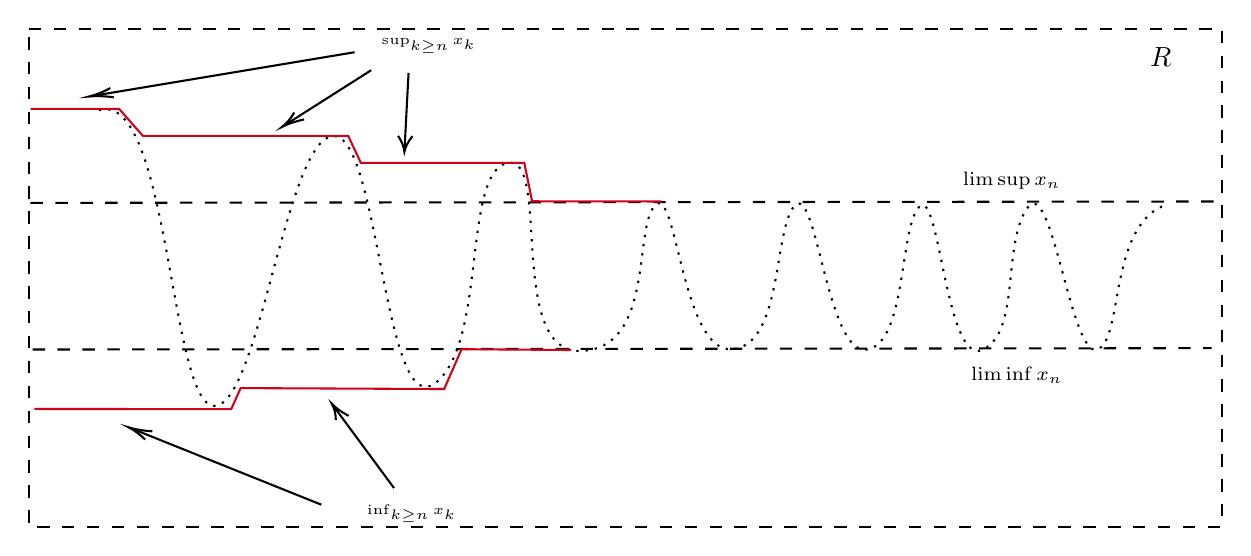
\begin{tikzpicture}[x=0.75pt,y=0.75pt,yscale=-1,xscale=1.5]
%uncomment if require: \path (0,472); %set diagram left start at 0, and has height of 472

%Curve Lines [id:da44573902991754766] 
\draw  [dash pattern={on 0.84pt off 2.51pt}]  (141.52,165.81) .. controls (164.19,155.81) and (164.19,308.48) .. (178.57,308.29) .. controls (192.95,308.1) and (201.52,180.48) .. (216.57,178.29) .. controls (231.62,176.1) and (232.95,316.76) .. (249.57,297.29) .. controls (266.19,277.81) and (258.19,196.48) .. (272.57,191.29) .. controls (286.95,186.1) and (272.29,282.77) .. (296.19,281.81) .. controls (320.09,280.85) and (313.07,223.21) .. (320.07,211.71) .. controls (327.07,200.21) and (328.62,283.28) .. (345,281) .. controls (361.38,278.72) and (358.07,222.21) .. (365.07,211.71) .. controls (372.07,201.21) and (375.37,284.12) .. (388.19,281.14) .. controls (401.01,278.16) and (398.57,221.71) .. (405.07,212.21) .. controls (411.57,202.71) and (413.52,290.14) .. (425.52,281.14) .. controls (437.52,272.14) and (431.57,231.21) .. (439.57,213.21) .. controls (447.57,195.21) and (453.65,285.77) .. (462.19,281.14) .. controls (470.73,276.52) and (465.52,219.81) .. (485,211) ;
%Straight Lines [id:da2292557377025013] 
\draw  [dash pattern={on 4.5pt off 4.5pt}]  (120.19,281.14) -- (498.86,280.48) ;
%Straight Lines [id:da021754386863272357] 
\draw  [dash pattern={on 4.5pt off 4.5pt}]  (119.52,210.48) -- (500.19,209.81) ;
%Straight Lines [id:da9184013042125718] 
\draw [color={rgb, 255:red, 208; green, 2; blue, 27 }  ,draw opacity=1 ]   (119.57,165.21) -- (148,165.21) -- (155.6,178.17) -- (221.57,178.21) -- (225.64,191.21) -- (278.14,191.21) -- (280.64,209.71) -- (322.19,209.81) ;
%Straight Lines [id:da2894532143841366] 
\draw [color={rgb, 255:red, 208; green, 2; blue, 27 }  ,draw opacity=1 ]   (120.8,309.77) -- (184,309.85) -- (187.02,299.72) -- (252.4,300.17) -- (258,280.97) -- (293.2,281.37) ;
%Straight Lines [id:da09981137612794089] 
\draw    (228.95,146.57) -- (201.73,172.52) ;
\draw [shift={(200.29,173.9)}, rotate = 316.36] [color={rgb, 255:red, 0; green, 0; blue, 0 }  ][line width=0.75]    (7.65,-2.3) .. controls (4.86,-0.97) and (2.31,-0.21) .. (0,0) .. controls (2.31,0.21) and (4.86,0.98) .. (7.65,2.3)   ;
%Straight Lines [id:da7736001528911756] 
\draw    (240.95,147.9) -- (239.69,183.91) ;
\draw [shift={(239.62,185.9)}, rotate = 272.01] [color={rgb, 255:red, 0; green, 0; blue, 0 }  ][line width=0.75]    (7.65,-2.3) .. controls (4.86,-0.97) and (2.31,-0.21) .. (0,0) .. controls (2.31,0.21) and (4.86,0.98) .. (7.65,2.3)   ;
%Straight Lines [id:da01875292146375851] 
\draw    (223.62,137.9) -- (140.23,158.75) ;
\draw [shift={(138.29,159.24)}, rotate = 345.96] [color={rgb, 255:red, 0; green, 0; blue, 0 }  ][line width=0.75]    (7.65,-2.3) .. controls (4.86,-0.97) and (2.31,-0.21) .. (0,0) .. controls (2.31,0.21) and (4.86,0.98) .. (7.65,2.3)   ;
%Straight Lines [id:da685154290163863] 
\draw    (212.95,355.9) -- (152.67,319.6) ;
\draw [shift={(150.95,318.57)}, rotate = 31.05] [color={rgb, 255:red, 0; green, 0; blue, 0 }  ][line width=0.75]    (7.65,-2.3) .. controls (4.86,-0.97) and (2.31,-0.21) .. (0,0) .. controls (2.31,0.21) and (4.86,0.98) .. (7.65,2.3)   ;
%Straight Lines [id:da47753478631845336] 
\draw    (236.29,347.9) -- (217.17,309.03) ;
\draw [shift={(216.29,307.24)}, rotate = 63.81] [color={rgb, 255:red, 0; green, 0; blue, 0 }  ][line width=0.75]    (7.65,-2.3) .. controls (4.86,-0.97) and (2.31,-0.21) .. (0,0) .. controls (2.31,0.21) and (4.86,0.98) .. (7.65,2.3)   ;
%Shape: Rectangle [id:dp6544720458561455] 
\draw  [dash pattern={on 4.5pt off 4.5pt}] (118.95,126.57) -- (502.29,126.57) -- (502.29,366.57) -- (118.95,366.57) -- cycle ;

% Text Node
\draw (418,194.3) node [anchor=north west][inner sep=0.75pt]  [font=\scriptsize]  {$\limsup x_{n}$};
% Text Node
\draw (420.67,288.3) node [anchor=north west][inner sep=0.75pt]  [font=\scriptsize]  {$\liminf x_{n}$};
% Text Node
\draw (231.33,129.97) node [anchor=north west][inner sep=0.75pt]  [font=\tiny]  {$\sup _{k\geq n} x_{k}$};
% Text Node
\draw (226.67,354.64) node [anchor=north west][inner sep=0.75pt]  [font=\tiny]  {$\inf_{k\geq n} x_{k}$};
% Text Node
\draw (478.14,134.26) node [anchor=north west][inner sep=0.75pt]    {$\mathbb{R}$};


\end{tikzpicture}
\end{tikznt}



Dada $\left(x_n\right)_{n \in \mathbb{N}}$ acotada en $\mathbb{R}$ existen $\alpha, \beta \in \mathbb{R}$ tales que $\alpha \leq x_n \leq \beta$ para todo $n \in \mathbb{N}$. Si $X_n=\left\{x_k: k \geq n\right\}$ tomamos
$$
\begin{aligned}
& b_n=\sup X_n, \mathrm{y} \\
& a_n=\inf X_n .
\end{aligned}
$$
De esta forma tenemos que
$$
\alpha \leq a_1 \leq a_2 \leq \cdots \leq a_{n-1} \leq a_n \leq \cdots \leq b_n \leq b_{n-1} \leq \cdots \leq b_1 \leq \beta .
$$

\begin{note}
Todo esto se tiene porque primero estamos en los reales y la sucesión es acotada, podemos garantizar el Sup y el Ínf, note que:\\

$$X_1=\{x_1,x_2,\ldots\} \quad \text{y}\quad X_2=\{x_2,x_3,\ldots\}$$

Luego $\sup X_1$ o es $x_1$ o está en $X_2$ y $\sup X_2$ o es $x_2$ o está en $X_3$, luego razonando de esta forma nos damos cuenta que $\sup X_n\leq \sup X_{n-1}$, por eso $b_n\leq b_{n-1}$.
\end{note}

\begin{note}
Todo esto pasa ya que el supremo es mayor o igual que todos los elementos de $X_n$, luego si el supremo de $X_n$ fuera $x_n$, entonces el supremo de $X_{n+1}$ sería más pequeño, y en caso de que no fuera $x_n$, entonces el supremo de $X_n$ y $X_{n+1}$ serían iguales.
\end{note}

Además todos estos $b_n=\sup X_n<\beta$ ya que la sucesión es acotada, para $a_n=\inf X_n$ se razona de la misma forma para llegar a que $a_n\leq a_{n+1}$, espero que esto sea suficiente para entender digamos un poco este tema, es algo que en un inicio cuesta, pero que entenderlo bien es muy muy clave, este tipo de aclaraciones Omar al menos la suele dar en clase, pero en este curso no todos los profesores son tan buenos. 



\begin{definition}
Definimos el límite inferior (denotado por líminf $x_n$ ) y el límite superior (notado por $\left.\operatorname{lim} \sup x_n\right)$ de $\left(x_n\right)_{n \in \mathbb{N}}$ como
$$
\begin{aligned}
& \liminf x_n=\sup a_n=\lim _{n \rightarrow \infty} a_n, \quad y \\
& \lim \sup x_n=\inf b_n=\lim _{n \rightarrow \infty} b_n .
\end{aligned}
$$    
\end{definition}

A continuación presentamos una definición un poco más chingona de límites superior e inferior, son equivalentes en realidad las definiciones, pero esta definición es agradable porque nos evita pensar en $X_n$ y desviar nuestra atención.

\begin{definition}

Definimos el límite inferior (denotado por liminf $x_n$ ) y el límite superior (notado por $\left.\operatorname{lim} \sup x_n\right)$ de $\left(x_n\right)_{n \in \mathbb{N}}$ como:

$$    \begin{aligned}
\lim \inf x_n & =\lim _{n \rightarrow \infty}\left(\inf _{k \geq n} x_k\right) \\
\lim \sup x_n & =\lim _{n \rightarrow \infty}\left(\sup _{k \geq n} x_k\right)
\end{aligned}$$

\end{definition}

No es difícil ver con la definición anterior que ambas son equivalentes, solo observe qué son $a_n$ y $b_n$ en la definición 1.

\subsection{Quiz 6:}

\end{itemize}

\begin{itemize}[leftmargin=*]
    \item  Sean $\left(a_n\right)$ sucesión acotada en $\left(\mathbb{R}^m, d_{\infty}\right)$ y $\left(b_n\right)$ una sucesión convergente en $\left(\mathbb{R}^m, d_2\right)$. Entonces $\left(a_n+b_n\right)$ es acotada en $\left(\mathbb{R}^m, d_2\right)$.\\

    \item Si la sucesión ( $\left.a_n\right)$ es convergente, con límite no nulo, en $\left(\mathbb{R}, d_2\right)$ y $a_{n+1}=2\left(a_n\right)^2-$ $a_{n-1}$ para $n \geq 3$, entonces $\operatorname{lim}_{n \rightarrow \infty} a_n=1$.\\

    \begin{proof}
    Tenemos que $(a_n)$ es convergente, luego:

    \begin{align*}
        a=\lim_{n \to \infty} a_n&=\lim_{n \to \infty} a_{n+1}\\
        &=2\lim_{n \to \infty}(a_n)^2-\lim_{n \to \infty} a_{n-1}\\
        &=2a^2-a\\
        &=a(2a-1)
    \end{align*}
    
    Entonces $(2a-1)=1$, por tanto $a=1$.
    \end{proof}


    \item Sean ( $E, d$ ) espacio métrico, $\left(a_n\right)$ y $\left(b_n\right)$ sucesiones en $(E, d)$. Si $a_n=b_n$ para $n \geq m$ con $m \in \mathbb{N} y\left(a_n\right)$ es convergente, entonces $\left(b_n\right)$ es convergente.\\

    \begin{proof}
    Tenemos que existe $m\in \N$ tal que $a_n=b_n$ para todo $n\geq m$, luego como $a_n$ es convergente, para todo $\epsilon>0$, existe un $N\in \N$ tal que si $n>\max\{N,m\}$, entonces:

    $$|b_n-a|=|a_n-a|<\epsilon$$

    Luego $b_n$ es convergente y además converge a $a$
    \end{proof}

\begin{note}
Usamos el máximo ya si $m$ es el máximo entonces a partir del punto en que $a_n=b_n$ ya tenemos convergencia, si $N$ es el máximo entonces desde antes de tener convergencia ya teníamos que $a_n=b_n$, luego es conveniente escoger $n>\max\{N,m\}$, para que se de $n$ en adelante tengamos tanto convergencia como que las sucesiones son iguales.
\end{note}
    
    \item Si la sucesión $\left(a_n\right)$ es convergente en $\left(\mathbb{R}^m, d_2\right)$, entonces $\left((-1)^n a_n\right)$ es convergente.\\
    
    Falso: Considere $(\R,d_1)$, (note que en $\R$, $d_2=d_1$), entonces si tomamos una sucesión constante, $(x_n)_{n\in\N}=(-1)^na_n$ no converge, por ejemplo: si $(a_n)_{n\in \N}=1$, entonces:

    $$(x_n)_{n\in \N}=\{-1,1,-1,1,-1,1,\ldots\}$$ 

    Vemos que $(x_n)_{n\in\N}$ no converge, para ello veamos que el límite superior no es igual al límite inferior\\

    Note que $\lim_{n \to \infty} \left( \inf_{k\geq n} x_k \right)=\lim_{n \to \infty} -a_n=\lim_{n \to \infty} -1=-1$ y por otro lado el \\
    $\lim_{n \to \infty} \left( \sup_{k\geq n} x_k\right)=\lim_{n \to \infty} a_n=\lim_{n \to \infty} 1=1$

    \item $\limsup \frac{(-1)^n}{n}=0$\\
    
    \begin{proof} 
    Observe que para todo $\epsilon>0$, existe $N\in \N$ tal que $\frac{1}{N}<\epsilon$, entonces si $n>N$:


    $$\left| \frac{1}{n} \right|<\epsilon$$

    Luego:

    $$\lim _{n \rightarrow \infty}\left(\sup _{k \geq n} \frac{(-1)^n}{n}\right)$$

    Veamos entonces quien es el $\sup_{k\geq n}\frac{(-1)^n}{n}$.

    \begin{align*}
        &\sup X_2=\sup \left\{\frac{1}{2},-\frac{1}{3},\frac{1}{4},\ldots\right\}\\
        &\sup X_3=\sup\left\{-\frac{1}{3},\frac{1}{4},-\frac{1}{5},\ldots\right\}\\
        &\sup X_4=\sup\left\{\frac{1}{4},-\frac{1}{5},\frac{1}{6},\ldots\right\}\\
        &\sup X_5=\sup\left\{-\frac{1}{5},\frac{1}{6},-\frac{1}{7},\ldots\right\}\\
        & \mathrel{\phantom{=askldfjaddsl}}\vdots
    \end{align*}

    Note que si $n$ es par entonces:

    $$\lim _{n \rightarrow \infty}\left(\sup_{k \geq n} \frac{(-1)^n}{n}\right)=\lim_{n \to \infty} \frac{1}{n}=0$$

    Si $n$ es impar:

    $$\lim _{n \rightarrow \infty}\left(\sup _{k \geq n} \frac{(-1)^n}{n}\right)=\lim_{n \to \infty} \frac{1}{2n+1}=0$$
    
    No es necesario probar este límite ya que probamos el caso general $\frac{1}{n}$ da 0.

    \end{proof} 


    \item  $\liminf \frac{(-1)^n n}{n+1}=1$.\\
 
 Falso: 

        $$\liminf \frac{(-1)^n n}{n+1}=\lim _{n \rightarrow \infty}\left(\inf_{k \geq n} \frac{(-1)^nn}{n+1}\right)$$

        Veamos entonces quién es el $\inf_{k\geq n} \frac{(-1)^nn}{n+1}$:

        \begin{align*}
            &\inf X_1=\inf \left\{-\frac{1}{2},\frac{2}{3},-\frac{3}{4},\ldots\right\}=-1\\
            &\inf X_2=\inf \left\{\frac{2}{3},-\frac{3}{4},\frac{4}{5},\ldots\right\}=-1\\
            &\inf X_3=\inf \left\{-\frac{3}{4},\frac{4}{5},-\frac{5}{6},\ldots\right\}=-1\\
            &\inf X_4=\inf \left\{\frac{4}{5},-\frac{5}{6},\frac{6}{7},\ldots\right\}=-1\\
            &\inf X_5=\inf \left\{-\frac{5}{6},\frac{6}{7},-\frac{7}{8},\ldots\right\}=-1\\
            & \mathrel{\phantom{=askaldfjasl}}\vdots
        \end{align*}

        Luego el $\inf_{k\geq n} \frac{(-1)^nn}{n+1}$ siempre es -1, por tanto:

        $$\liminf \frac{(-1)^n n}{n+1}=\lim _{n \rightarrow \infty}\left(\inf_{k \geq n} \frac{(-1)^nn}{n+1}\right)=\lim_{n \to \infty} -1=-1$$




    \item $\lim _{n \rightarrow \infty}(\sqrt{n+1}-\sqrt{n})=0$.\\
 
    Primero note que:

    $$\sqrt{n+1}-\sqrt{n} \left(\frac{\sqrt{n+1}+\sqrt{n}  }{\sqrt{n+1}+\sqrt{n} } \right)=\frac{1}{\sqrt{n+1}+\sqrt{n}}<\frac{1}{2\sqrt{n}}$$


    \begin{proof}
    
    Para todo $\epsilon>0$ existe un  $N\in  \N$ tal que $N>\frac{1}{4\epsilon^2}$, luego si $n>N$:

        $$\left|\frac{1}{2\sqrt{n} }\right|<\left|\frac{1}{2\sqrt{N} }\right|<\left|\frac{1}{2\sqrt{\frac{1}{4\epsilon^2}} }\right|=\epsilon$$


Luego en efecto $\lim_{n \to \infty} \sqrt{n+1}-\sqrt{n}=0   $
    \end{proof}

    

    \item Si $A, B \subseteq \mathbb{R}^n$ entonces $\overline{A+B}=\bar{A}+\bar{B}$\\
    
     Falso: Contraejemplo: Sea $A=\{(x,e^x) : x\in \R\}$ y $B=\{(y,0): y\in \R\}$, luego note que $\overline{B}=B$ y $\overline{A}=A$.

    $$A+B=\{(z,e^w): z,w\in \R\}=\{(x,y): x,y\in \R, y>0 \}$$

    Luego $\overline{A+B}=\{(x,y):x,y\in \R,y\geq0\}\neq\overline{A}+\overline{B}$

\item Si $(a_n)$ es una sucesión de números reales positivos, entonces
\begin{align*}
    \liminf_{n\to \infty} \frac{a_{n+1}}{a_n}\leq \liminf_{n \to \infty} \sqrt[n]{a_n}\leq \limsup_{n\to \infty} \sqrt[n]{a_n}\leq \limsup_{n\to \infty} \frac{a_{n+1}}{a_n}.
\end{align*}
\begin{proof}
    Póngale cuidado que esto es fino. Note que la desigualdad del medio es trivial, así que vamos a probar las desigualdades de los extremos.
    \begin{itemize}
        \item Vamos a empezar con la de la derecha porque tengo problemas psicológicos. Si $\displaystyle \limsup_{n\to \infty}\frac{a_{n+1}}{a_n}=\infty$, la desigualdad de la derecha se tiene de manera trivial. Supongamos que $\displaystyle \limsup_{n\to \infty}\frac{a_{n+1}}{a_n}=U<\infty$, entonces para todo $\epsilon>0$, existe $N\in \mathbb{Z}^+$, tal que si $n>N$, entonces 
        \begin{align*}
            \frac{a_{n+1}}{a_n}<U+\epsilon,
        \end{align*}
        Entonces, para $n>N$ y $m \in \mathbb{Z}^+$, se tiene $a_{n+m}<a_n(U+\epsilon)^m$ ¿por qué? Pues vamos a ver si me acuerdo. Dado $m \in \mathbb{Z}^+$ y $n>N$, tenemos
        \begin{align*}
            \frac{a_{n+1}}{a_n}<U+\epsilon, \hspace{5mm} \frac{a_{n+2}}{a_{n+1}}<U+\epsilon, \hspace{5mm} \dotsb \hspace{5mm}, \frac{a_{n+m}}{a_{n+m-1}}<U+\epsilon.
        \end{align*}
        Entonces tenemos que 
        \begin{align*}
            a_{n+1}&<a_n(U+\epsilon)\\
            \frac{a_{n+2}}{a_{n+1}}&<U+\epsilon,
        \end{align*}
        Multiplicando las dos desigualdades, se obtiene
        \begin{align*}
            a_{n+2}<a_n(U+\epsilon)^2.
        \end{align*}
        Análogamente, ahora tomamos las desigualdades
        \begin{align*}
            a_{n+1}&<a_n(U+\epsilon)\\
            \frac{a_{n+3}}{a_{n+2}}&<U+\epsilon,
        \end{align*}
        multiplicando se obtiene
        \begin{align*}
            a_{n+3}<a_n(U+\epsilon)^3.
        \end{align*}
        Realizando este proceso $m$ veces, obtenemos que
        \begin{align*}
            a_{n+m}<a_n(U+\epsilon)^m,
        \end{align*}
        y tomando la potencia $\dfrac{1}{n+m}$ a ambos lados se obtiene
        \begin{align*}
            (a_{n+m})^{\frac{1}{n+m}}<\left(a_n(U+\epsilon)^m\right)^{\frac{1}{n+m}}=(a_n)^{\frac{1}{n+m}}(U+\epsilon)^{\frac{m}{n+m}},
        \end{align*}
        de esta manera
        \begin{align*}
            \limsup_{m\to \infty} \left(a_{n+m}\right)^{\frac{1}{n+m}}\leq \limsup_{m\to \infty}(a_n)^{\frac{1}{n+m}}(U+\epsilon)^{\frac{m}{n+m}}=U+\epsilon
        \end{align*}
        Esto último porque $a_n>0$ para todo $n$ y $\displaystyle \lim_{m\to \infty}\sqrt[m]{a}=1$ para todo $a>0$ y del hecho de que $\displaystyle \lim_{m\to \infty}\frac{m}{n+m}=1$, luego
        \begin{align*}
            \limsup_{m\to \infty}(a_{n+m})^{\frac{1}{n+m}}=\limsup_{n\to \infty}\sqrt[n]{a_n}\leq U+\epsilon=\left(\limsup_{n\to \infty} \frac{a_{n+1}}{a_n}\right)+\epsilon,
        \end{align*}
        como $\epsilon$ es arbitrario y hay finitos $k$ menores que $N$, obtenemos
        \begin{align*}
            \limsup_{n\to \infty}\sqrt[n]{a_n}\leq \limsup_{n\to \infty} \frac{a_{n+1}}{a_n}
        \end{align*}

            \item Ahora, vamos a probar la desigualdad de la izquierda. Sea $\displaystyle\liminf_{n\to \infty}\frac{a_{n+1}}{a_n}=u$, por definición, dado $\epsilon>0$, existe $N\in \mathbb{Z}^+$ tal que si $n>N$, entonces
            \begin{align*}
                u-\epsilon<\frac{a_{n+1}}{a_n}.
            \end{align*}
            Nuevamente, realizando un procedimiento análogo al anterior, dados $n>N$ y $m \in \mathbb{Z^+}$ tenemos
            \begin{align*}
                (u-\epsilon)^ma_n\leq a_{n+m},
            \end{align*}
            luego
            \begin{align*}
                (u-\epsilon)^{\frac{m}{n+m}}(a_n)^{\frac{1}{n+m}}<(a_{n+m})^{\frac{1}{n+m}},
            \end{align*}
            de manera que
            \begin{align*}
                u-\epsilon=\liminf_{m\to \infty}(u-\epsilon)^{\frac{m}{n+m}}(a_n)^{\frac{1}{n+m}}\leq \liminf_{m\to \infty}(a_{n+m})^{\frac{1}{n+m}}.
            \end{align*}
            es decir,
            \begin{align*}
                u-\epsilon=\left(\liminf_{n\to \infty} \frac{a_{n+1}}{a_n}\right)-\epsilon\leq \liminf_{m\to \infty}(a_{n+m})^{\frac{1}{n+m}}=\liminf_{n\to \infty}\sqrt[n]{a_n}
            \end{align*}
            Nuevamente, como $\epsilon$ es arbitrario y hay finitos $k$ menores que $N$, tenemos que
            \begin{align*}
                \liminf_{n\to \infty} \frac{a_{n+1}}{a_n}\leq \liminf_{n\to \infty}\sqrt[n]{a_n}
            \end{align*}
    \end{itemize}
    

\end{proof}


\end{itemize}


\section{Completez}

\subsection{Algunos ejercicios al lector}

\begin{itemize}[leftmargin=*]
    \item Si $(x_n)$ es una sucesión convergente, entonces $(x_n)$ es una sucesión de Cauchy.\\

    \begin{proof}
    Sea $(x_n)$ una sucesión convergente, entonces para todo $\epsilon>0$, existe $N\in \N$ tal que si $n,m>N$, entonces $d(x_n,L)<\frac{\epsilon}{2}$ y $d(x_m,L)<\frac{\epsilon}{2}$. Así:

    $$d(x_n,x_m)\leq d(x_n,L)+d(L,x_m)<\frac{\epsilon}{2}+\frac{\epsilon}{2}=\epsilon$$
    \end{proof}

    \item Si $(x_n)$ es una sucesión de Cauchy, entonces toda subsucesión también es de Cauchy.\\

    \begin{proof}
        Sea $(x_n)$ una sucesión de Cauchy, entonces para todo $\epsilon>0$, existe $N\in \N$ tal que si $m,n\geq N$, $d(x_n,x_m)<\epsilon$.\\

        Considere $(x_{n_k})$ una subsucesión de $(x_n)$, luego como $n_k\geq k$, para todo $k\in \N$, en efecto si $L,M\geq k\geq N$ entonces $n_L,n_M\geq N$ y como $(x_n)$ es de Cauchy:

        $$d(x_{n_L},x_{n_M})<\epsilon$$ 
    \end{proof}

    \item Sea $(X,d)$ un espacio métrico. Una función $f:X \longrightarrow X$ se dice una contracción en $X$, si existe una constante $K \in (0,1)$ tal que $d(f(x),f(y))\leq Kd(x,y)$ para todo $x,y \in X$. Sea $x_0 \in X$ cualquiera y $x_n=f(x_{n-1})$ para $n \in \mathbb{Z}^+$. Muestre que si $f$ es una contracción, la sucesión $(x_n)$ es de Cauchy.\\
    
    \begin{proof}
      Sea $x_0 \in X$ cualquiera y la sucesión $(x_n)$ definida por $x_n=f(x_{n-1})$. Sean $m,n \in \mathbb{N}$ y, sin pérdida de generalidad, supongamos
      %que ella a mi siempre me trasnocha y que yo la pienso a toda hora%.
      que $n>m$. Tenemos que 
      \begin{align*}
          d(x_m,x_n)=d(f(x_{m-1}),f(x_{n-1}))&\leq Kd(x_{m-1},x_{n-1}),\\
          &\leq K^2d(x_{m-2},x_{n-2}),\\
          &\vdots\\
          &\leq K^md(x_0,x_{n-m}).
      \end{align*}
      Ahora, note que 
      \begin{align*}
          d(x_0,x_{n-m})&\leq d(x_0,x_1)+d(x_1,x_{n-m}),\\
          &\leq d(x_0,x_1)+Kd(x_0,x_{n-m-1}),\\
          &\leq d(x_0,x_1)+Kd(x_0,x_1)+Kd(x_1,x_{n-m-1}),\\
          &\leq d(x_0,x_1)+Kd(x_0,x_1)+K^2d(x_0,x_{n-m-2}),\\
          &\vdots\\
          &\leq d(x_0,x_1)+Kd(x_0,x_1)+K^2d(x_0,x_1)+\dotsb +K^{n-m-1}d(x_0,x_1),\\
          &=(1+K+K^2+\dotsb +K^{n-m-1})d(x_0,x_1),\\
          &=\left(\sum_{j=0}^{n-m-1} K^j\right)d(x_0,x_1).
      \end{align*}
      Usando la identidad 
      \begin{align*}
          \sum_{j=0}^{N} x^j=\frac{1-x^{N+1}}{1-x}, \hspace{2mm} x\neq 0,1,
      \end{align*}
      tenemos que
      \begin{align*}
          d(x_m,x_n)&\leq K^md(x_0,x_{n-m}),\\
          &\leq K^m\left(\frac{1-K^{n-m}}{1-K}\right)d(x_0,x_1)\\
          &=\frac{K^m-K^n}{1-K}d(x_0,x_1).
      \end{align*}
      Ahora, como $K \in (0,1)$, es fácil ver que la función $K^x$ tiende a $0$ cuando $x$ tiende a infinito. Por tanto, para todo $\epsilon>0$ existe $N \in \mathbb{N}$ tal que si $n>N$, entonces $K^n<\epsilon$. Tomando $ \displaystyle \epsilon_1=\frac{1-K}{2d(x_0,x_1)}\epsilon$, con $\epsilon>0$, existe $M \in \mathbb{N}$ tal que si $n,m >M$, entonces, $K^m,K^n<\epsilon_1$. De esta manera
      \begin{align*}
          d(x_m,x_n)&\leq\frac{K^m-K^n}{1-K}d(x_0,x_1),\\
          &\leq \frac{K^m+K^n}{1-K}d(x_0,x_1),\\
          &< \frac{2\epsilon_1}{1-K}d(x_0,x_1),\\
          &=\frac{2d(x_0,x_1)}{1-K}\cdot \frac{1-K}{2d(x_0,x_1)}\epsilon =\epsilon.
      \end{align*}
      Así, concluimos que la sucesión $(x_n)$ es de Cauchy.
    \end{proof}
    \begin{note}
        Cuando el espacio métrico es un espacio completo, esto implica que la sucesión anterior es convergente. Es posible mostrar que, el punto $p$ al que converge esta sucesión, es un punto fijo de la función $f$ (es decir, $f(p)=p$) y además, este es único. Este resultado es conocido como el Teorema del Punto Fijo de Banach, o Teorema de Contracción de Banach.
    \end{note}
\end{itemize}



\subsection{Quiz 7:}

\begin{itemize}[leftmargin=*]
    
    \item $\mathbb{Z}$ es completo con la métrica usual.\\

    \begin{proof}
        Sea $(x_n)$ una sucesión de Cauchy en $(\Z,d_1)$, luego para todo $\epsilon>0$, existe $N\in \N$ tal que si $n,m\geq N$, entonces:

        $$|x_n-x_m|<\epsilon$$

        Por tanto $x_n=x_m$, es decir $(x_n)$ es eventualmente constante, entonces $\lim_{n \to \infty} x_n=x_m$, como $x_m \in \Z$, acabamos.
    \end{proof}

    \item Toda sucesión de Cauchy en $\mathbb{Z}$ con la métrica discreta es convergente.\\
    
    Veamos un resultado más elegante. Sea $(X,d_d)$ donde $d_d$ es la métrica discreta, entonces $X$ es completo.\\

    \begin{proof}
        Sea $(x_n)$ una sucesión de Cauchy en $(X,d_d)$, entonces para todo $\epsilon>0$, existe $N\in\N$ tal que si $m,n\geq N$, entonces:

        $$d_d(x_n,x_m)<\epsilon$$

        Sea $\epsilon=\frac{1}{2}$, entonces:

        $$d_d(x_n,x_m)<\frac{1}{2}$$

        Entonces $x_n=x_m$, luego $(x_n)$ es eventualmente constante, por tanto converge en $X$.
    \end{proof}

    \item $\mathbb{Q}$ no es completo con la métrica usual.\\

    \begin{proof}
        Supongamos que $\Q$ es completo. Considere una sucesión $(x_n)$ convergente definida en $\Q$, entonces es de Cauchy y como $\Q$ es completo, entonces $(x_n)$ converge en $\Q$, luego $\Q$ es cerrado, contradicción.
    \end{proof} 

    \item  Si $\left(a_n\right)$ es de Cauchy en $\left(\mathbb{R}^m, d_2\right)$ y $\left(b_n\right)$ es convergente en $\left(\mathbb{R}^m, d_2\right)$, entonces $\left(a_n+\right.$ $b_n$ ) es de Cauchy.\\

    \begin{proof}
        Sabemos que $(\R^m,d_2)$ es completo, luego si $(a_n)$ es de Cauchy, entonces es convergente, tenemos que $(b_n)$ es convergente, por tanto $(a_n+b_n)$ es convergente, y toda sucesión convergente es de Cauchy.
    \end{proof}

    \item  $\left(\mathbb{R}^n, d_{\infty}\right)$ es un espacio métrico completo.\\

    \begin{proof}
        Sabemos que $(R^m,d_2)$ es completo, luego si $(x_n)$ es una sucesión de Cauchy en $(\R^m,d_{\infty})$, para todo $\epsilon>0$, existe $N\in \N$ tal que si $n>N$:

        $$d_{\infty}(x_n,L)<\frac{\epsilon}{m}$$

        Luego como $md_{\infty}(x,y)\geq d_2(x,y)$:

        $$d_{2}(x_n,L)\leq md_{\infty}(x_n,L)<m\frac{\epsilon}{m}=\epsilon$$

        i.e. $(\R^m,d_{\infty})$ es completo.
    \end{proof}
\end{itemize}


\section{Compacidad}

Aquí toca tener particular cuidado con el teorema de Bolzano y sus implicaciones, pero también con la prueba que se presenta de Heine-Borel. Es muy importante a la hora de hacer los ejercicios tener claras todas las equivalencias que se dan al final del capítulo.



\subsection{Quiz 8:}

\begin{itemize}[leftmargin=*]
    \item Sean $(E, d)$ espacio métrico y $F \subset E$. Si todo cubrimiento por conjuntos cerrados de $F$ admite un subcubrimiento finito, entonces $F$ es compacto.\\

    \begin{proof}
    Supongamos que todo cubrimiento de $F$ por conjuntos cerrados admite un subcubrimiento finito, entonces en particular el cubrimiento:

    $$F\subseteq\bigcup_{x \in E}\{x\} 
        $$

     Admite un subcubrimiento finito, luego el conjunto $F$ es finito y todo conjunto finito es compacto.
    \end{proof}

    \item 
El conjunto $(0,1]$ no es compacto en $\mathbb{R}$ con la métrica usual.\\

    \begin{proof}
    Considere el cubrimiento:

    $$(0,1]\subseteq\bigcup_{i=1}^{\infty} 
        \left(\frac{1}{n},2\right)$$

    Note que este cubrimiento abierto no admite un subcubrimiento finito.\\

    Note que por Heine-Borel esto es trivial.
    \end{proof}

    \item Todo conjunto totalmente acotado es completo.\\

    Falso: Considere el intervalo $(0,1)$ en $(\R,d_1)$, este conjunto totalmente acotado en $\R$ ya que es acotado, pero no es completo porque no es cerrado.

    \item Todo conjunto completo es totalmente acotado.\\
    
    Falso: $(R,d_1)$ es completo, pero no es acotado y por tanto no es totalmente acotado.

    \item Todo espacio métrico secuencialmente compacto es completo. \\

    \begin{proof}
    Sea $(X,d)$ un espacio métrico y $(x_n)$ una sucesión de Cauchy en $(X,d)$, como $(X,d)$ es secuencialmente compacto, $(x_n)$ tiene una subsucesión convergente, como $(x_n)$ es de Cauchy y tiene una subsucesión convegente, converge.
    \end{proof}

    \item Todo espacio métrico completo es compacto.
    
    Falso: Note que $(\R,d_1)$ es completo, pero no es compacto por Heine-Borel

    \item Todo subconjunto cerrado y acotado de un espacio métrico es compacto. \\ 
    
    Falso: Sea $(\R,d_d)$ donde $d_d$ es la métrica discreta, luego $\R$ es cerrado y acotado ya que $\R\subseteq B(0,2)$, note que el cubrimiento de abiertos:

    $$\R\subseteq \bigcup_{i \in \R}\{x\}$$

        No admite un subcubrimiento finito.
\end{itemize}
 
\begin{note}
No te preocupes si no entiendes la prueba de Heine-Borel, de hecho muy pocas veces un ejercicio de parcial será tan fácil como usar ese teorema, lo que yo recomendaría sería entender bien todos los conceptos aquí plasmados, en particular el teorema de Bolzano y las equivalencias presentadas al final de la sección.
\end{note}

\begin{note}
A continuación presentamos una serie de ejercicios tanto de parciales anteriores como algunos que se nos van ocurriendo junto con su solución, claramente los invitamos a pensar cómo resolverlos antes de leerlos aquí.
\end{note}


\subsection{Ejercicios adicionales:}


Esto es como una clase de preparación para lo que sería un segundo parcial.\\

\textbf{Para cada una de las siguientes afirmaciones diga si es falso o verdadero, si es verdadero escriba la demostración y si es falso de el contraejemplo, si la afirmación dice demuestre pues esa sí demuéstrela xd:}

\begin{itemize}[leftmargin=*]

\item Sea (X,d) un espacio métrico, si $S\subseteq X$ es acotado entonces es totalmente acotado:\\

Falso: Considere $(\R,d_d)$ los reales con la métrica discreta, luego $\R$ es acotado ya que $\R\subseteq B(0,2)$, pero $\R$ no es totalmente acotado ya que si $\epsilon=\frac{1}{2}$, no existe $A=\{a_1,a_2,\ldots,a_n\}$, tal que 

$$R\subseteq \bigcup_{i=1}^nB\left(a_i,\frac{1}{2}\right)=\bigcup_{i=1}^n\{a_i\} 
    =A 
    $$

    ya que de lo contrario $\R$ sería finito.


\item Sea $\R$ con la métrica usual, entonces $\limsup(a_n+b_n)=\limsup(a_n)+\limsup(b_n)$:\\

Falso: Sean $(a_n)=(-1)^n$ y $(b_n)=-(-1)^n$, luego $\limsup(a_n+b_n)=\lim _{n \rightarrow \infty}\left(\sup _{k \geq n} 0\right)=0$, pero $\lim _{n \rightarrow \infty}\left(\sup _{k \geq n} (-1)^n\right)=\lim _{n \rightarrow \infty}\left(\sup _{k \geq n} -(-1)^n\right)=1$, luego $\limsup(a_n)+\limsup(b_n)=2$ y $2\neq 0$.

\item Sea $(X,d)$ un espacio métrico y $A,C\subseteq X$, si $A\subseteq C\subseteq \overline{A}$, entonces para todo $c\in C$ y para todo $r>0$, $B(c,r)\cap A\neq \emptyset$:\\

\begin{proof}
Sea $c\in C$, entonces $c\in \overline{A}$, luego $c$ es un punto adherente, es decir para todo $r>0$, $B(c,r)\cap A\neq \emptyset$.
\end{proof}

\item Sea $(X,d)$ un espacio métrico y $A,C\subseteq X$, entonces $(A\cup C)^{\prime}=A^{\prime}\cup C^{\prime}$:\\

\begin{proof}

\begin{align*}
(A\cup C)^{\prime}&=\{x\in X: \text{para todo }r>0, (B(x,r)\setminus \{x\})\cap (A\cup C)\neq \emptyset\}\\
&=\{x\in X: \text{para todo }r>0, ((B(x,r)\setminus \{x\})\cap A \cup (B(x,r)\setminus \{x\})\cap C) \neq \emptyset\}\\
&=A^{\prime}\cup C^{\prime}
\end{align*}

\end{proof}

\item Sea $(X,d)$ un espacio métrico, si $S\subseteq X$, entonces $(S^{\prime})^{\prime}=S^{\prime}$.\\

Falso: Sea $S=\left\{\frac{1}{n}: n\in \Z^+\right\}$, entonces $S^{\prime}=\{0\}$ y $(S^{\prime})^{\prime}=\emptyset$.\\

\item Demuestre que si $(X,d)$ es un espacio métrico completo y $Y\neq \emptyset$ es un subconjunto cerrado de $X$, entonces $(Y,d_y)$ es completo.\\

\begin{proof}
Sea $(x_n)$ una sucesión de Cauchy definida en $Y$, entonces $(x_n)$ converge en $X$ ya que $(X,d)$ es completo, por tanto $(x_n)$ es una sucesión convergente definida en $Y$ y $Y$ es cerrado si y solo si toda sucesión convergente definida en $Y$ converge en $Y$, por tanto $(x_n)$ converge en $Y$, es decir $(Y,d_y)$ es completo.
\end{proof}

\item Se $(X,d)$ es un espacio métrico completo, entonces $(X,d^{\prime})$ con $d^{\prime}(x,y)=\dfrac{d(x,y)}{1+d(x,y)}$ es completo.\\

\begin{proof}
Sea $(x_n)$ una sucesión de Cauchy en $X$, entonces como $(X,d)$ es completo, existe $N\in \N$ tal que si $n>N$:

$$d(x_n,L)<\epsilon$$

Note que:

$$\dfrac{d(x_n,L)}{1+d(x_n,L)}\leq d(x_n,L)<\epsilon$$

Luego $(x_n)$ también converge en $(X,d^{\prime})$, por tanto $(X,d^{\prime})$ es completo.
\end{proof}

\item Demuestre que si $(X,d)$ es un espacio métrico y $\{x,y,u,v\}\subseteq X$, entonces:

$$|d(x,v)-d(y,u)|\leq d(x,y)+d(u,v)$$

\begin{proof}
Supongamos que $d(x,v)-d(y,u)<0$, luego:

\begin{align*}
 |d(x,v)-d(y,u)|&=d(y,u)-d(x,v)\\
 &\leq d(y,x)+d(x,u)-d(x,v)\\
 &\leq d(y,x)+d(x,v)+d(v,u)-d(x,v)\\
 &=d(x,y)+d(u,v)  
\end{align*}

Ahora si $d(x,v)-d(y,u)\geq0$, entonces:

\begin{align*}
|d(x,v)-d(y,u)|&=d(x,v)-d(y,u)\\
&\leq d(x,y)+d(y,v)-d(y,u)\\ :
&\leq d(x,y)+d(y,u)+d(u,v)-d(y,u)\\
&=d(x,y)+d(u,v)
\end{align*}
\end{proof}

\begin{note}
Note que esto fue aplicar desigualdad triangular varias veces pero de la forma adecuada.
\end{note}

\end{itemize}

\section{Conexidad}

\begin{note}
Muchos teoremas en cálculo requieren de conexidad en su hipótesis, por eso es importante este capítulo, nos ayuda a formalizar y entender la idea de conexidad sobre al menos espacios métricos. Como bien lo dicen las notas, esto intuitivamente se puede pensar como que el conjunto es un solo pedazo en caso sea conexo, en este capítulo al menos no hay mucho que decir, pasemos a los ejercicios.
\end{note}

\subsection{Quiz 9}

\begin{itemize}[leftmargin=*]

\item El espacio métrico $(\Z,d_1\mid_{\Z\times \Z})$ es conexo:\\

Falso: Sea $A=\{0\}$, note que $B(0,1)=\{0\}$, luego $A$ es abierto, Ahora observe que $A$ es cerrado ya que su complemento es abierto.

\item $\R$ con la métrica discreta es conexo:\\

Falso: Nuevamente $A=\{0\}$ es abierto y cerrado al tiempo.

\item Si $A$ es conexo en $(\R^n,d_2)$, entonces $A$ es conexo en $(\R_n,d_1)$\\


\begin{proof}
 Sabemos que $d_1$ y $d_2$ son métricas equivalentes en $\mathbb{R}^n$, es decir, que un conjunto es abierto en $(\mathbb{R}^n,d_2)$ si y sólo si es abierto en $(\mathbb{R}^n,d_1)$. Supongamos que $A$ es conexo en $(\mathbb{R}^n,d_2)$ y no es conexo en $(\mathbb{R}^n,d_1)$. Como $A$ no es conexo en $(\mathbb{R}^n,d_1)$, existen $X,Y$ abiertos en $(\mathbb{R}^n,d_1)$ tales que $X \cup Y=A$ y $X \cap Y=\emptyset$. Como $X,Y$ son abiertos en $(\mathbb{R}^n,d_1)$, también lo son en $(\mathbb{R}^n,d_2)$, luego, $A$ no es conexo en $(\mathbb{R}^n,d_2)$. Contradicción.
\end{proof}



\item Si $X\subseteq \R$ es conexo con la métrico usual entonces $\R\setminus X$ es conexo con la métrica usual:

Falso: Obviamente los singleton son conexos, por ejemplo $\{0\}$ es conexo, pero $\R\setminus\{0\}$ ya no lo es, note que:

$$\R=(-\infty,0)\cup (0,\infty)$$

Dos abiertos y disyuntos distintos de vacío.

\item Si $A\subseteq \R$ es conexo con la métrica usual, entonces $A\setminus \{a_1,\ldots,a_n\}$ donde $a_i\in A$ para todo $i$ es conexo.

Falso: Considere $A=(-1,1)$ conexo en $\mathbb{R}$ con la métrica usual, y considere $A-\{0\}=(-1,0)\cup (0,1)$, luego $A-\{0\}$ es unión de abiertos disyuntos en $\mathbb{R}$ con la métrica usual, por lo tanto no es conexo

\item Sean $(E,d)$ un espacio métrico y $A\subseteq E$, si $A$ es conexo, entonces $int(A)$ es conexo.\\

Falso: Considere $(E,d)=(\mathbb{R}^2,d_2)$ y sea $A=B[-1;1]\cup B[1;1]$ conexo. Note que $int(A)=B(-1,1)\cup B(1,1)$, luego $int(A)$ es unión de abiertos disyuntos en $(\mathbb{R}^2,d_2)$ y por lo tanto no es conexo

\item Sean $(E,d)$ un espacio métrico y $A\subseteq E$, si $int(A)$ es conexo entonces $A$ es conexo.\\

Falso: Sea $(\R,d_1)$, recuerde que $int(\N)=\emptyset$, que es conexo, pero $\N$ no es conexo ya que no es un intervalo.
\end{itemize}


\section{Ejercicios 3:}
\begin{itemize}[leftmargin=*]
    \item Sea $V$ un espacio vectorial sobre $\mathbb{R}$. Una aplicación 
        \begin{align*}
            ||\cdot||:&V \longrightarrow \mathbb{R}\\
            &x \longmapsto ||x||
        \end{align*}
        se denomina norma si:
        \begin{enumerate}[(1)]
            \item Para todo $x \in V$, $||x||\geq 0$ y $||x||=0$ si y sólo si $x=0$.
            \item Para todo $ \in V$ y todo $\lambda \in \mathbb{R}$, $||\lambda x||=|\lambda|||x||$.
            \item Para todo $x,y \in V$, $||x+y||\leq ||x||+||y||$.
        \end{enumerate}
        Demuestre que si $(V,||\cdot||)$ es un espacio vectorial normado, entonces $(V,d)$ es un espacio métrico con 
        \begin{align*}
            d:&V \times V \longrightarrow \mathbb{R}\\
            &(x,y) \longmapsto d(x,y)=||x-y||.
        \end{align*}
        \begin{enumerate}[a)]
            \item A fin de que una métrica de un espacio vectorial real $V$ provenga de una norma es necesario y suficiente que dados $x,y,z \in V$ y $\lambda \in \mathbb{R}$, $d(x+z,y+z)=d(x,y)$ y $d(\lambda x,\lambda y)=|\lambda|d(x,y)$.
            \item Demuestre que todas las normas de $\mathbb{R}^n$ son equivalentes, es decir, dadas $||\cdot||_1$ y $||\cdot||_2$ normas en $\mathbb{R}^n$, existen $c,d>0$ tales que $c||x||_2\leq ||x||_1\leq d||x||_2$ para todo $x \in \mathbb{R}^n$.
        \end{enumerate}

        \begin{solution}
            Sea $(V,||\cdot||)$ un espacio vectorial normado y $d(x,y):=||x-y||$ para $x,y \in V$.
            \begin{itemize}
                \item Si $d(x,y)=0$, por definición $||x-y||=0$, por tanto $x-y=0$, es decir, $x=y$, recíprocamente, si $x=y$, $d(x,y)=||x-y||=||0||=0$.
                \item $d(x,y)=||x-y||=||-(y-x)||=|-1|\cdot||y-x||=||y-x||=d(y,x)$.
                \item Sean $x,y,z \in V$, entonces
                \begin{align*}
                    d(x,y)=||x-y||=||x-z+(z-y)||\leq ||x-z||+||z-y||=d(x,z)+d(z,x).
                \end{align*}
            \end{itemize}
            de esta manera, $d$ define una métrica en $V$
            \begin{enumerate}[(a)]
                \item Supongamos que $d$ es una métrica en $V$ que proviene de una norma, es decir, existe $||\cdot||$ norma en $V$ tal que $d(x,y)=||x-y||$ para todo $x,y \in V$. Sean $x,y,z \in V$, entonces
                \begin{align*}
                    d(x+z,y+z)=||(x+z)-(y+z)||=||x-y||=d(x,y).
                \end{align*}
                Si $\lambda \in \mathbb{R}$, entonces
                \begin{align*}
                    d(\lambda x,\lambda y)=||\lambda x-\lambda y||=||\lambda(x-y)||=|\lambda|\cdot||x-y||=|\lambda|d(x,y).
                \end{align*}
                De manera recíproca, supongamos que $d$ es una métrica en $V$ tal que para todo $x,y,z \in V$ y $\lambda \in \mathbb{R}$ se tiene $d(x+z,y+z)=d(x,y)$ y $d(\lambda x,\lambda y)=|\lambda|d(x,y)$. Para $x \in V$, definimos $||x||:=d(x,0)$ ($0$ el elemento neutro de la suma en el espacio vectorial $V$). Veamos que $||\cdot||$ define una norma en $V$.
                \begin{itemize}
                    \item $||x||\geq 0$ por definición de métrica. Supongamos que $||x||=0$, esto quiere decir que $||x||=d(x,0)=0$, como $d$ es métrica, esto quiere decir que $x=0$. De manera recíproca, si $x=0$, $||x||=d(x,0)=d(0,0)=0$.

                    \item Si $\lambda\in \mathbb{R}$, tenemos 
                    \begin{align*}
                        ||\lambda x||=d(\lambda x,0)=d(\lambda x,\lambda 0)=|\lambda|d(x,0)=|\lambda|\cdot ||x||.
                    \end{align*}

                    \item Si $x,y \in V$, tenemos
                    \begin{align*}
                        ||x+y||=d(x+y,0)\leq d(x+y,y)+d(y,0)=d(x,0)+d(y,0)=||x||+||y||.
                    \end{align*}
                \end{itemize}
                es decir, $||\cdot||$ define una norma en $V$. Sólo resta ver que $d(x,y)=||x-y||$ para todo $x,y \in V$, pero esto es inmediato ya que
                \begin{align*}
                    d(x,y)=d((x-y)+y,y)=d(x-y,0)=||x-y||.
                \end{align*}

                \item Considere $A=\{||\cdot||:\mathbb{R}^n\to [0,\infty):||\cdot|| \text{ es una norma en } \mathbb{R}^n\}$ y definimos la relación en $A$ dada por 
                \begin{align*}
                    ||\cdot||_1 \sim ||\cdot||_2 \hspace{5mm} \Longleftrightarrow \hspace{5mm} \text{existen } c_1,c_2\in \mathbb{R}^+ \text{ tales que } c_1||x||_2\leq ||x||_1\leq c_2||x||_2 \text{ para todo } x \in \mathbb{R}^n.
                \end{align*}
                veamos que la relación $\sim$ es una relación de equivalencia en $A$.
                \begin{itemize}
                    \item \textbf{Reflexividad:} Sea $||\cdot||\in A$, entonces $||x||\leq ||x||\leq ||x||$, es decir, tomando $c_1=c_2=1$, se tiene que $||\cdot||\sim ||\cdot||$.
                    \item \textbf{Simetría:} Sean $||\cdot||_1, ||\cdot||_2 \in A$ tal que $||\cdot||_1\sim ||\cdot||_2$, por definición, existen $c_1,c_2 \in \mathbb{R}^+$ tales que $c_1||x||_2\leq ||x||_1\leq c_2||x||_2$ para todo $x \in \mathbb{R}^n$. Dado $x \in \mathbb{R}^n$, tenemos que $c_1||x||_2\leq ||x||_1$, como $c_1>0$, $||x||_2\leq \dfrac{1}{c_1}||x||_1$. Análogamente, como $||x||_1\leq c_2||x||_2$, tenemos $\dfrac{1}{c_2}||x||_1\leq ||x||_2$. Entonces definiendo $C_1:=\dfrac{1}{c_2}$ y $C_2:=\dfrac{1}{c_1}$, tenemos
                    \begin{align*}
                        C_1||x||_1\leq ||x||_2\leq C_2||x||_2,
                    \end{align*}
                    para todo $x \in \mathbb{R}^n$, es decir, $||\cdot||_2\sim ||\cdot||_1$.
                    \item \textbf{Transitividad:} Sean $||\cdot||_1,||\cdot||_2,||\cdot||_3 \in A$ tales que $||\cdot||_1\sim ||\cdot||_2$ y $||\cdot||_2\sim ||\cdot||_3$. Por definición, existen $c_1,c_2,c_3,c_4 \in \mathbb{R}^+$ tales que
                    \begin{align*}
                        c_1||x||_2\leq ||x||_1\leq c_2 ||x||_2\\
                        c_3||x||_3\leq ||x||_2\leq c_4||x||_3,
                    \end{align*}
                    la segunda cadena de desigualdades se escribe como
                    \begin{align*}
                        c_3||x||_3\leq ||x||_2 \hspace{5mm} \text{ y } \hspace{5mm} ||x||_2\leq c_4||x||_3
                    \end{align*}
                    dado que $c_1,c_2$ son positivos, multiplicando cada una de estas desigualdades, se obtiene
                    \begin{align*}
                        c_1c_3||x||_3\leq c_1||x||_2\\
                        c_2||x||_2\leq c_2c_4||x||_3,
                    \end{align*}
                    por tanto, si definimos $C_1:=c_1c_3$ y $C_2:=c_2c_4$, tenemos
                    \begin{align*}
                        C_1||x||_3\leq c_1||x||_2\leq ||x||_1\leq c_2||x||_2\leq C_2||x||_3,
                    \end{align*}
                    para todo $x \in \mathbb{R}^n$ y por tanto, $||\cdot||_1\sim ||\cdot||_3$.
                \end{itemize}
                de esta manera, tenemos que $\sim$ es una relación de equivalencia en $A$. Ahora, es claro que 
                \begin{align*}
                    ||\cdot||_t:\mathbb{R}^n&\longrightarrow \mathbb{R}\\
                    x=(x_1,...,x_n)&\longmapsto ||x||_t:=\sum_{k=1}^n|x_k|
                \end{align*}
                define una norma en $\mathbb{R}^n$. Sea $||\cdot||\in A$ cualquiera y $\mathcal{B}=\{e_1,...,e_n\}$ la base canónica de $\mathbb{R}^n$. Dado $x=(x_1,...,x_n) \in \mathbb{R}^n$, la expresión como combinación lineal en la base $\mathcal{B}$ es 
                \begin{align*}
                    x=x_1e_1+\dotsb+x_ne_n=\sum_{k=1}^nx_ke_k,
                \end{align*}
                de manera que, al ser $||\cdot||$ una norma
                \begin{align*}
                    ||x||=\left|\left|\sum_{k=1}^nx_ke_k\right|\right|\leq \sum_{k=1}^n||x_ke_k||=\sum_{k=1}^n|x_k|\cdot||e_k||
                \end{align*}
                Si tomamos $\displaystyle C_2=\max_{1\leq k\leq n} ||e_k||$, tenemos
                \begin{align*}
                    ||x||\leq \sum_{k=1}^n|x_k|\cdot||e_k||\leq C_2\sum_{k=1}^n |x_k|=C_2||x||_t.
                \end{align*}
                Ahora, queremos mostrar que existe una constante positiva $C_1$ tal que $C_1||x||_t\leq ||x||$ para todo $x \in \mathbb{R}^n$ y así concluir que $||\cdot||\sim ||\cdot||_t$. Note que esto es equivalente a que exista $C_1>0$ tal que $||x||\geq C_1$ para todo $x \in \mathbb{R}^n$ tal que $||x||_t=1$. En efecto, si existe $C_1>0$ tal que $C_1||x||_t\leq ||x||$ para todo $x \in \mathbb{R}^n$, si $||x||_t=1$, esto es $C_1\leq ||x||$. Recíprocamente, si $||x||\geq C_1$ para todo $x \in \mathbb{R}^n$ con $||x||_t=1$, con $C_1>0$, tomemos $y \in \mathbb{R}^n$ con $y\neq 0$, entonces $x=\dfrac{y}{||y||_t}$ cumple que $||x||_t=1$, por tanto $||x||\geq C_1$, pero siendo $||\cdot||$ una norma
                \begin{align*}
                    ||x||=\left|\left|\frac{y}{||y||_t}\right|\right|=\frac{1}{||y||_t}\cdot||y||\geq C_1\\
                    \Rightarrow ||y||\geq C_1||y||_t.
                \end{align*}
                Entonces, si tomamos $S=\{x \in \mathbb{R}^n:||x||_t=1\}$, por la continuidad de las normas (ejercicio), la función $||\cdot||:S\to \mathbb{R}$ es continua y además, $S$ es compacto, entonces la función $||\cdot||$ alcanza mínimo en el conjunto $S$, es decir, existe $z\in S$ tal que $||x||\geq ||z||$ para todo $x \in \mathbb{R}^n$. Como $||z||_t=1$, $z\neq 0$ y por tanto $||z||>0$, entonces tomando $C_1=|z|$, se obtiene el resultado. De esta manera, una norma arbitraria $||\cdot||$ está relacionada con la norma $||\cdot||_t$, pero al ser $\sim$ una relación de equivalencia, quiere decir que la clase de equivalencia de $||\cdot||_t$ es todo $A$, por tanto, cualesquiera dos normas en $\mathbb{R}^n$ son equivalentes.
            \end{enumerate}
        \end{solution}
    \item Si $(E,d)$ es un espacio métrico, defina
    \begin{align*}
        d': &E \times E \longrightarrow \mathbb{R}\\
        &(x,y) \longmapsto d'(x,y)=\frac{d(x,y)}{1+d(x,y)}.
    \end{align*}
    Demuestre que $(E,d')$ es un espacio métrico.\\
    
    \begin{proof}
    Verifiquemos las condiciones para que $d'$ sea una métrica.
        \begin{itemize}
            \item Veamos que $d'(x,y)=0$ si y sólo si $x=y$. En efecto, supongamos que $d'(x,y)=0$, por definición, $\displaystyle \frac{d(x,y)}{1+d(x,y)}=0$, de donde se deduce que $d(x,y)=0$. Como por hipótesis $d$ es métrica, entonces $x=y$. Si $x=y$, es trivial que $d'(x,y)=0$.
            \item Ahora, veamos que $d'(x,y)=d'(y,x)$ para todo $x,y \in E$. Como $d$ es métrica, tenemos que $d(x,y)=d(y,x)$ para todo $x,y \in E$. esto implica que dados $x,y \in E$
            \begin{align*}
                d'(x,y)=\frac{d(x,y)}{1+d(x,y)}=\frac{d(y,x)}{1+d(y,x)}=d'(y,x),
            \end{align*}
            lo cual prueba la propiedad.
            \item Veamos que para todo $x,y,z \in E$, se tiene que $d'(x,y)\leq d'(x,z)+d'(z,y)$. Para esto, primero veamos que, dados $a,b\geq 0$, si $a \leq b$, entonces $\displaystyle \frac{a}{1+a}\leq \frac{b}{1+b}$, en efecto
            \begin{align*}
                a&\leq b\\
                \Rightarrow a + ab &\leq b+ab,\\
                \Rightarrow a(1+b) &\leq b(1+a),\\
                \Rightarrow \frac{a}{1+a}&\leq \frac{b}{1+b}.
            \end{align*}
            Ahora, como $d$ es métrica, sabemos que para todo $x,y,z \in E$, $d(x,y)\leq d(x,z)+d(z,y)$, usando el resultado anterior, tenemos que para todo $x,y,z \in E$
            \begin{align*}
                d'(x,y)=\frac{d(x,y)}{1+d(x,y)}&\leq \frac{d(x,z)+d(z,y)}{1+d(x,z)+d(z,y)}\\
                &=\frac{d(x,z)}{1+d(x,z)+d(z,y)}+\frac{d(z,y)}{1+d(x,z)+d(z,y)}.
            \end{align*}
            Como $d(x,z),d(z,y)\geq 0$, es claro que
            \begin{align*}
                1+d(x,z)\leq 1+d(x,z)+d(z,y),\\
                1+d(z,y) \leq 1+d(x,z)+d(z,y).
            \end{align*}
            Por lo tanto,
            \begin{align*}
                \frac{d(x,z)}{1+d(x,z)+d(z,y)}\leq \frac{d(x,z)}{1+d(x,z)},\\
                \frac{d(z,y)}{1+d(x,z)+d(z,y)}\leq \frac{d(z,y)}{1+d(z,y)}.
            \end{align*}
            De esta manera
            \begin{align*}
                d'(x,y)=\frac{d(x,y)}{1+d(x,y)}&\leq \frac{d(x,z)}{1+d(x,z)+d(z,y)}+\frac{d(z,y)}{1+d(x,z)+d(z,y)},\\
                &\leq \frac{d(x,z)}{1+d(x,z)}+\frac{d(z,y)}{1+d(z,y)}=d'(x,z)+d'(z,y),
            \end{align*}
            lo cual completa la demostración.
        \end{itemize}
        
    \end{proof}

    \item Pruebe que en $(\mathbb{R},d_1)$:
    \begin{enumerate}[a)]
        \item $\displaystyle \lim_{n \rightarrow \infty} \sqrt[n]{n}=1$.\\

        \begin{proof} Note que si $n\geq 1$, entonces $\sqrt[n]{n}=1+a_n$ con $a_n\geq 0$, luego:

        \begin{align*}
            n&=(1+a_n)^n=\sum_{i=0
            }^n\binom{n}{i}1^{n-i}a_n^i,\\
            &=1+n a_n+\dfrac{n(n-1)}{2}a_n^2+\ldots+a_n^n,\\
            &\geq \dfrac{n(n-1)}{2}a_n^2,\\
            &\geq 0.
        \end{align*}

De esto se sigue que $0\leq \dfrac{n(n-1)}{2}a_n^2\leq n$, es decir $0\leq a_n\leq \sqrt{\dfrac{2}{n-1}}$, sabemos que $\lim_{n\to \infty}\dfrac{1}{\sqrt{n-1}}=0$, luego:

$$0\leq \lim_{n\to \infty}a_n\leq \sqrt{2}\lim_{n\to \infty}\dfrac{1}{\sqrt{n-1}}=0.$$

Luego como $a_n$ tiende a 0, es claro que el límite es 1.
        
        \end{proof}
        
        \item $\displaystyle \lim_{n \rightarrow \infty} \frac{\nu(n)}{n}=0$, 
        donde $\nu(n)$ es el número de divisores primos de $n$.\\

        \begin{proof}
            Sea  $\tau(n)=\displaystyle\sum_{j\mid n}1$, en efecto $0\leq  v(n)\leq\tau(n)$, para todo $n\in \Z^+$, ahora note que $\tau(n)\leq 2\sqrt{n}$, ya que para cada divisor de $n$ menor igual que $\sqrt{n}$ hay exactamente un divisor mayor igual que $\sqrt{n}$, es decir, si $j\mid n$ y $j\leq \sqrt{n}$, entonces $\dfrac{n}{j}\geq \sqrt{n}$ y además $\dfrac{n}{j}\mid n$. Luego:

            \begin{align*}
                0\leq \lim_{n\to \infty} \dfrac{v(n)}{n}\leq \lim_{n\to\infty}\dfrac{2\sqrt{n}}{n}=0
            \end{align*}
        \end{proof}
        
        \item La sucesión
        \begin{align*}
            \left(\frac{1}{2},\cfrac{1}{2+\cfrac{1}{2}},\cfrac{1}{2+\cfrac{1}{2+\cfrac{1}{2}}},...\right)
        \end{align*}
        es convergente.\\

        \begin{proof}
            Esta demostración es fina, pero sólo se le ocurre a uno después de estar en un estado de desesperación considerable.
            
            Note que
            \begin{align}
                \sqrt{2}=1+\frac{1}{\sqrt{2}+1}
            \end{align}
            Aplicando nuevamente la identidad (1.1) en el $\sqrt{2}$ que aparece en el denominador, tenemos
            \begin{align*}
                \sqrt{2}&=1+\cfrac{1}{\sqrt{2}+1}\\
                &=1+\cfrac{1}{1+\cfrac{1}{\sqrt{2}+1}+1}\\
                &=1+\cfrac{1}{2+\cfrac{1}{\sqrt{2}+1}}
            \end{align*}
            Realizando repetidamente este proceso, obtenemos
            \begin{align*}
                \sqrt{2}-1&=\cfrac{1}{\sqrt{2}+1},\\
                &=\cfrac{1}{2+\cfrac{1}{\sqrt{2}+1}},\\
                &=\cfrac{1}{2+\cfrac{1}{2+\cfrac{1}{\sqrt{2}+1}}},\\
                &\vdots\\
                &=\cfrac{1}{2+\cfrac{1}{2+\cfrac{1}{\ddots 2+ \cfrac{\empty}{2+\cfrac{1}{\sqrt{2}+1}}}}},
            \end{align*}
            que asintóticamente, es la misma sucesión que estamos considerando. Luego, la sucesión original converge y lo hace a $\sqrt{2}-1$.\\
        \end{proof}

        \begin{proof}
            \textbf{Alternativa} Esta demostración no es tan fina, pero es más aterrizada. 

            Note que la sucesión, se puede escribir de manera recursiva como $a_{n+1}=\dfrac{1}{2+a_{n}}$ para $n \in \mathbb{Z}^+$, con $a_1=\dfrac{1}{2}$. Es claro que $a_n \geq 0$ para todo $n \in \mathbb{Z}^+$, entonces $2+a_n\geq 2$ y así $\dfrac{1}{2}\geq\dfrac{1}{2+a_n}$. Esto acaba de probar que $0\leq a_n \leq \dfrac{1}{2}$ para todo $n \in \mathbb{Z}^+$, en otras palabras, la sucesión está contenida en $\left[0,\dfrac{1}{2}\right]$. 

            Ahora, considere $\left(\left[0,\dfrac{1}{2}\right],d_1\right)$ como subespacio métrico de $\mathbb{R}$ y considere la función $f$ definida en  $\left(\left[0,\dfrac{1}{2}\right],d_1\right)$ como
            \begin{align*}
                f(x)=\frac{1}{2+x}.
            \end{align*}
            Es claro que la sucesión $(a_n)$ se puede escribir como $a_1=\dfrac{1}{2}$ y $a_{n+1}=f(a_n)$ para $n \in \mathbb{Z}^+$. Note además que la función $f$ es decreciente en $\left[0,\dfrac{1}{2}\right]$, por lo tanto, para todo $x \in \left[0,\dfrac{1}{2}\right]$, se tiene $\dfrac{2}{5}=f\left(\dfrac{1}{2}\right)\leq f(x) \leq f(0)=\dfrac{1}{2}$. Esto quiere decir que $Im (f)=\left[\dfrac{2}{5},\dfrac{1}{2}\right] \subseteq \left[0,\dfrac{1}{2}\right]$. Esto está un poquito enredado, pero esperen que es importante. 

            Ahora, note que dados $x,y \in \left[0,\dfrac{1}{2}\right]$, tenemos que
            \begin{align*}
                d_1(f(x),f(y))=\left|\frac{1}{2+x}-\frac{1}{2+y}\right|=\left|\frac{y-x}{(2+x)(2+y)}\right|.
            \end{align*}
            Por lo que probamos antes, $f(x)=\dfrac{1}{2+x}\leq \dfrac{1}{2}$, y lo mismo sucede con $f(y)=\dfrac{1}{2+y}$, entonces
            \begin{align*}
                d_1(f(x),f(y))=\left|\frac{y-x}{(2+x)(2+y)}\right|\leq \frac{1}{4}|x-y|=\frac{1}{4}d_1(x,y).
            \end{align*}
            En resumen
            \begin{align*}
                f: \left(\left[0,\dfrac{1}{2}\right],d_1\right) \longrightarrow \left(\left[0,\dfrac{1}{2}\right],d_1\right)\\
            \end{align*}
            es tal que $d_1(f(x),f(y))\leq \dfrac{1}{4}d_1(x,y)$ para todo $x,y \in \left[0,\dfrac{1}{2}\right]$, es decir, dado que $\dfrac{1}{4} \in (0,1)$, $f$ es una contracción en $\left(\left[0,\dfrac{1}{2}\right],d_1\right)$. Por el tercer ejercicio de la \textbf{Sección 1.4.1}, tenemos que la sucesión $a_{n+1}=f(a_n)$ es de Cauchy. Además, como $\left[0,\dfrac{1}{2}\right]$ es compacto, entonces $\left(\left[0,\dfrac{1}{2}\right],d_1\right)$ es completo y por tanto, la sucesión $(a_n)$ converge.
        \end{proof}
    \end{enumerate}
    \item Sean $(x_n)_{n \in \mathbb{N}}$ y $(y_n)_{n \in \mathbb{N}}$ sucesiones acotadas en $(\mathbb{R},d_1)$, y tomemos $a=\liminf x_n$, $A=\limsup x_n$, $b=\liminf y_n$ y $B=\limsup y_n$. Demuestre que 
    \begin{enumerate}[a)]
        \item $\limsup (x_n +y_n)\leq A+B$.
        \item $\limsup(-x_n)=-a$.
        \item $\liminf (x_n+y_n)\geq a+b$.
        \item $\liminf(-x_n)=-A$.
        \item $\liminf(x_n \cdot y_n)\geq ab$.
    \end{enumerate}
    
    \item Encuentre el interior, la clausura, la frontera, los puntos de acumulación en $(\mathbb{R}, d1)$ de los siguientes conjuntos:
    \begin{enumerate}[a)]
        \item $\displaystyle A=\left\{\frac{1}{n}:n \in \mathbb{Z}^+\right\}$.
        \begin{solution}
            \begin{itemize}
                \item \textbf{Interior.} Note que en $(\mathbb{R},d_1)$, los conjuntos abiertos deben ser no contables o ser vacío, por tanto, dado que $A$ es contable, no puede contener un conjunto abierto no vacío, es decir, $Int(A)=\emptyset$.
                \item \textbf{Puntos de Acumulación}. Note que $A \subseteq (0,1]$ y que además, todos los puntos de $A$ son aislados, es decir, $A \cap A'= \emptyset$. Ahora, haciendo uso de la propiedad arquimediana de $\mathbb{R}$, sabemos que para todo $\epsilon>0$, existe $n \in \mathbb{Z}^+$ tal que $\displaystyle \frac{1}{n}<\epsilon$. Esto quiere decir que $\displaystyle \left| \frac{1}{n}-0\right|=d\left(\frac{1}{n},0\right)<\epsilon$, luego $0 \in A'$. Sabiendo que para todo $x \in (-\infty,0)\cup (1,\infty)$, la distancia a $A$ es siempre mayor que $0$, se tiene que $x\notin A'$. Así, $A'=\{0\}$.
                \item \textbf{Clausura.} Usando el hecho de que $\overline{A}=A\cup A'$, tenemos que $\overline{A}=A\cup \{0\}$.
                \item \textbf{Frontera.} Usando el hecho de que $\overline{A}=Int(A)\cup \partial A$, como $Int(A)=\emptyset$, entonces $\partial A=\overline{A}=A\cup \{0\}$.
            \end{itemize}
        \end{solution}
        \item $\displaystyle B=\left\{\frac{1}{n}+\frac{1}{m}:n,m \in \mathbb{Z}^+\right\}$.
        \begin{solution}
            \begin{itemize}
                \item \textbf{Interior.} Nuevamente, dado que $B$ es un conjunto contable, tenemos que $Int(B)=\emptyset$.
            \end{itemize}
        \end{solution}
        \item $\mathbb{Q}$.
        \item $\mathbb{I}$.
        \item $[a,b)$.
        \item $\{2^{-n}+5^{-m}:n,m \in \mathbb{Z}^+\}$.
    \end{enumerate}
    \item Dados $S,T$ subconjuntos de un espacio métrico $(E,d)$, pruebe que 
    \begin{enumerate}[a)]
        \item $Int(S\cap T)=Int(S)\cap Int(T)$.\\

        \begin{proof}
            El caso en que $Int(S \cap T)$ o $Int(S)\cap Int(T)$ son vacíos, verifican la propiedad de manera relativamente fácil.
            
            Sea $x \in Int(S \cap T)$, por definición, existe $r>0$ tal que $B(x;r) \subseteq S \cap T$. Como $S \cap T \subseteq S$ y $S \cap T \subseteq T$, entonces $B(x;r) \subseteq S$ y $B(x;r) \subseteq T$, es decir, $x \in Int(S)$ y $x \in Int(T)$, o lo que es lo mismo $x \in Int(S) \cap Int(T)$. Así, hemos probado que $Int(S \cap T)\subseteq Int(S) \cap Int(T)$.

            Ahora, sea $y \in Int(S) \cap Int(T)$, por definición, $y \in Int(S)$ y $y \in Int(T)$, de esta manera, existen $r_1,r_2>0$ tales que $B(y;r_1)\subseteq S$ y $B(y;r_2)\subseteq T$. Considere $r=\min\{r_1,r_2\}$, luego $B(y;r)\subseteq B(y;r_1)$ y $B(y;r) \subseteq B(y;r_2)$. De esta manera, $B(y;r) \subseteq S \cap T$, es decir, $y \in Int(S \cap T)$. Hemos probado, entonces, que $Int(S) \cap Int(T) \subseteq Int(S \cap T)$, lo cual completa la demostración.
        \end{proof}
        
        \item $Int(S) \cup Int(T) \subseteq Int(S \cup T)$.\\
        
        \begin{proof}
            Igual que antes, dejamos al lector verificar el caso cuando es vacío.

            Sea $x \in Int(S) \cup Int(T)$, por definición, $x \in Int(S)$ o $x \in Int(T)$. Veremos solamente el caso en el que $x \in Int(S)$, ya que el otro caso es análogo y lo puede desarrollar el lector con la idea que prosigue.

            Si $x \in Int(S)$, entonces existe $r>0$ tal que $B(x;r) \subseteq S$. Como $S \subseteq S \cup T$, entonces $B(x;r)\subseteq S \cup T$, es decir, $x \in Int(S \cup T)$. Luego $Int(S) \cup Int(T) \subseteq Int(S \cup T)$.
        \end{proof}
        
        \item $\overline{S\cap T}\subseteq \overline{S}\cap \overline{T}$.\\

        \begin{proof}
            Tomemos $x \in \overline{S\cap T}$, por definición, para todo $r>0$, $B(x;r)\cap (S\cap T) \neq \emptyset$. Usando la conmutatividad y asociatividad de la intersección entre conjuntos, tenemos que $(B(x;r)\cap S)\cap T\neq \emptyset$ y $(B(x;r)\cap T)\cap S\neq \emptyset$, esto implica que $B(x;r)\cap S\neq \emptyset \neq \emptyset$ y $B(x:r)\cap T\neq \emptyset$ y como $r$ es arbitrario, concluimos que $x \in \overline{S}$ y $x \in \overline{T}$.
        \end{proof}
        \item $S'$ es cerrado.\\
        
        \begin{proof}
            Esta demostración está en la sección 3.3 de las notas, sin embargo, vamos a realizar una prueba alternativa que, si se comprende bien, deja muy claro el concepto de derivado. Denotamos por $B^*(x;r)=B(x;r)\setminus \{x\}$. Vamos a mostrar que $(S')^c=E\setminus S'$ es un conjunto abierto. Tomemos $y \in (S')^c$, por definición, existe $r>0$ tal que $B^*(y;r)\cap S= \emptyset$, o lo que es lo mismo, $B(y;r)\cap S \subseteq \{y\}$. Veamos que $B(y;r) \subseteq (S')^c$.

            Por contradicción, supongamos que $B(y,r)\cap S' \neq \emptyset$, entonces existe $x \in B(y,r)\cap S'$. Como $x \in S'$, para todo $r'>0$, $B^*(x;r')\cap S \neq \emptyset$, además, como $x \in B(y;r)$ y las bolas abiertas son conjuntos abiertos, existe $r_1>0$ tal que $B(x;r_1)\subseteq B(y;r)$. Ahora, como $y \notin S'$, entonces $x\neq y$, por tanto, $r_2=d(x,y)>0$ y sea $R=\min\{r_1,r_2\}$. Es claro que $B^*(x;R)\subseteq B(x;R) \subseteq B(y;r)$, entonces $B^*(x;R)\cap S \subseteq B(y;r)\cap S \subseteq \{y\}$, esto es una contradicción, ya que $y \notin B^*(x;R)$, lo cual implicaría que $B^*(x;R)\cap S = \emptyset$, lo que contradice el hecho de que $x \in S'$. De esta manera $B(y;r) \subseteq (S')^c$ y, dado que fue $y$ fue tomado de manera arbitraria, concluimos que $(S')^c$ es un conjunto abierto, es decir, $S'$ es cerrado. 
        \end{proof}
        \item $(S \cup T)'=S'\cup T'$.\\
        
        \item $(\overline{S})'=S'$\\

    \end{enumerate}

            \item Si $X \subseteq \mathbb{R}^n$ es no contable muestre que $X \cap X^{\prime} \neq \phi$ y $X^{\prime}$ es no contable
        
        \item Un conjunto $V \subset \mathbb{R}^n$ es convexo, si dados $u, v \in V$, entonces $t u+(1-t) v \in V$ para todo $t \in[0,1]$. Considerando $\left(\mathbb{R}^n, d_2\right)$ demuestre que:
        
        \begin{itemize}
            \item Las bolas abiertas de $\left(R^n, d_2\right)$ son convexos de $\mathbb{R}^n$.
            
            \item El interior de un convexo, es convexo.
            
            \item La clausura de un convexo, es convexo.
            \end{itemize}

        \item Sea $(M, d)$ espacio métrico. Si $S, A \subset M$ son tales que $A \subset S \subset \bar{A}$, decimos que $A$ es denso en $S$.
        
        \begin{itemize}
        
        \item Considerando $\left(\mathbb{R}^n, d_2\right)$, pruebe que $\mathbb{Q}^n$ es denso en $\mathbb{R}^n$.
        
        \item Si $A$ es denso en $S$ y $B$ es abierto en $S$, muestre que $B \subset \overline{A \cap B}$.
        
    \end{itemize}
    
    \item Sea $(E, d)$ un espacio métrico.Si todo conjunto infinito de $E$ tiene un punto de acumulación en $(E, d)$ muestre que existe $B \subseteq E$ contable y $\bar{B}=E$ ( es decir $E$ es separable). Sugerencia:muestre que para $\delta_n=\frac{1}{n}$ existen $x_1^{(n)} \cdots, x_l^{(n)} \in E$ tales que $d\left(x_i^{(n)}, x_j^{(n)}\right)>\frac{1}{n}$ si $i \neq j$ y que $E=\cup B\left[x_i^{(n)}, \frac{1}{n}\right]$

    \item Consideremos $\left(\mathbb{R}^n, d_2\right)$. Un subconjunto $S \subset \mathbb{R}^n$ es perfecto si $S^{\prime}=S$. Pruebe que si $S$ es perfecto, entonces $S$ no es enumerable. Sugerencia: use el teorema de Baire

    \item Demuestre que el conjunto de Cantor es perfecto en $\left(\mathbb{R}, d_1\right)$.
    
    \item Sean $\left(\mathbb{R}^n, d_2\right)$ y $X \subseteq \mathbb{R}^n$. Muestre que todo cubrimiento abierto de $X$ admite un subrecubrimiento contable (Lindelöf).Sugerencia considere el conjunto $\{B(q, r)$ : $\left.q \in \mathbb{Q}^n, r \in \mathbb{Q}\right\}$
    
    \item Sean $U$ abierto en $(E, d)$ y $\left\{K_i\right\}_{i \in \mathbb{N}}$ una familia de compactos de $(E, d)$ tales que $K_1 \supset K_2 \supset K_3 \supset \cdots$. Si $K=\bigcap_{i \in \mathbb{N}} K_i \subset U$, entonces existe $i \in \mathbb{N}$ tal que $K_i \subset U$.
    
    \item Sean $(E, d)$ espacio métrico, $S, T \subset E$ tales que $S$ es cerrado y $T$ es compacto. Demuestre que $S \cap T$ es compacto.\\
    \begin{proof}
        Como $T$ es compacto, entonces $T$ es cerrado, y como $S$ también lo es $S\cap T$ es cerrado. Ahora, como $S\cap T \subseteq T$, y $T$ es compacto, entonces $S \cap T$ también es compacto, por ser un subconjunto cerrado de un compacto. 
    \end{proof}
    
    \item Sean $(E, d)$ espacio métrico y $X, Y \subset E$. Si $X$ es conexo y $X \subset Y \subset \bar{X}$, entonces $Y$ es conexo. Concluya en particular que la adherencia de un conjunto conexo es conexo.\\
    \begin{proof}
        Por contradicción, supongamos que $Y$ no es conexo, entonces, por definición, existen $A$ y $B$ abiertos no vacíos en $Y$, tales que $A\cap B=\emptyset$ y $A \cup B=Y$. Como $X$ es conexo y $X \subseteq Y$, entonces se debe tener que $X \subset A$ o $X \subset B$. Sin pérdida de generalidad, supongamos que $X \subset A$. Como $B$ es abierto, para todo $b \in B$, existe $r>0$ tal que $B(b;r) \subset B$, esto quiere decir que $B(b;r)\cap A=\emptyset$ y por tanto, $B(b;r)\cap X=\emptyset$. Así, para todo $b \in B$, se tiene que $b \notin \overline{X}$, lo cuál contradice que $Y \subset \overline{X}$. Así, $Y$ debe ser conexo. 

        En particular, note que si $X$ es un conjunto conexo, es trivial que $X \subset \overline{X} \subset \overline{X}$. Por el resultado anterior, se puede concluir que $\overline{X}$ es conexo.
    \end{proof}

    \item Describa todos los conjuntos conexos y enumerables de $\left(\mathbb{R}^n, d_2\right)$.
    
    \item Sean $C, X$ subconjuntos de un espacio métrico $(E, d)$. Si $C$ es conexo y tiene puntos en común con $X$ y con $E \backslash X$, entonces muestre que algún punto de $C$ pertenece a la frontera de $X$.
\end{itemize}




